\chapter{\uppercase{Design Dataset and Experiments}}\label{Ch:Model_Training}

In this chapter, we will discuss the Dataset Design, Training and Experiments done in this project. The Dataset Design steps started from acquisition and encoding including the essential pre-processing steps, and the justification for their need. Pre-processing steps are data extraction, data cleansing, data format, data encoding techniques used. Also, it contains comparisons between the three techniques used. The training phase started by exploring what the ratio of Training, Testing, and Validation is. Choosing the correct percentage of training dataset compared to the Testing and Validation in Deep learning differs from normal machine learning structure, and it affects the model performance. The results and Discussion phase It explains the results of all the 192 experiments on our dataset. Also, How we assess our model design.

\clearpage

\section{Dataset Design}

In this section, We introduces the Dataset acquisition and encoding including the essential pre-processing steps, and the justification for their need. Pre-processing steps are data extraction, data cleansing, data format, and data encoding techniques used. Also, it contains comparisons between the three techniques used.

The collection of the dataset was one of the most laborious tasks in this project. There were criteria we were searching to find. These criteria are as follows,
\begin{itemize}
  
  \item \textbf{Datasets availability:} There are old Arabic references which have a lot of Poems but not all these books were not available in a PDF or a Web pages format, and it was hard to find it.
  
  \item \textbf{The Poem with diacritics:} There are resources which have Arabic Poems, but it is much harder to find same with diacritics.
  
  \item \textbf{The amount of the dataset:} To have a successful project with good results we need a massive amount of data. From the previous work, We did not find this amount of data. The maximum number found was 1.5k. However, We were searching for around 1.5M record of classified poetry.

  
  \item \textbf{Cleansing of this data:} There was a limitation for the datasets which we can consider it, or we can scrap it due to the limitation for the APIs or the ready datasets in this context.
  
\end{itemize}
To meet the above criteria and overcome it, We applied following,

\begin{itemize}

  \item \textbf{Datasets availability:} We have scrapped the Arabic datasets from two big poetry websites: \textarabic{الديوان}~\cite{diwan}, \textarabic{الموسوعة الشعرية}~\cite{PoetryEncyclopedia2016}. Both merged into one large dataset, and we open sourced it online ~\cite{ArabicpoetryDS}.

  \item \textbf{The Poem with diacritics:} We tried to get the most verses with the available diacritics, but the diacritics states are not consistent, So, a verse can be fully diacritics, Semi diacritics or without diacritics.

  \item \textbf{The amount of the dataset:} The total number of verses is 1,862,046 poetic verses; each verse labeled by its meter (class), the poet who wrote it, and the age which it was written. There are 22 meters, 3701 poets and 11 ages; and they are Pre Islamic, Islamic, Umayyad, Mamluk, Abbasid, Ayyubid, Ottoman, Andalusian, the era between Umayyad and Abbasid, Fatimid and modern. We are only interested in the 16 classic meters which attributed to Al-Farahidi, and they are the majority of the dataset with a total number of 1,722,321 verses. Figure~\ref{Fig:Data_Size_Distribution} shows the distribution of the verses per meter. %@@@ add datasets figures percentage per class
  
  \item \textbf{Cleansing of this data:} Dataset was not cleaned enough for usage in this research, but we have applied cleansing rules explained in details in Data Preparation and Cleansing section~\ref{sec:Data_Clens}. We also open sourced all the code scripts used in our online repository~\cite{HCILAB_ArabicPoetry_2018}.
\end{itemize}

\begin{figure}[!t]
  \centering
  \begin{tikzpicture}
    \begin{axis}[
    symbolic x coords={Taweel,
   Kamel,
   Baseet,
   Khafeef,
   Wafeer,
   Rigz,
   Raml,
   Motakarib,
   Sar'e,
   Monsareh,
   Mogtath,
   Madeed,
   Hazg,
   Motadarik,
   Moktadib,
   Modar'e
    },
    xtick=data,
    % the following x label positioning does work here.
    every axis y label/.style= {at={( 0.15, 1.07)}, anchor=north},
    ylabel style={font=\footnotesize},
    xticklabel style = {font=\footnotesize},
    ylabel={Verses},
    height=8cm,
    x=0.4cm,
    x tick label style={rotate=90, anchor=east},
    enlarge y limits=0.07,
    name=left plot,%
    title=(a) \textit{Arabic Dataset},%
    title style={at={(0.5,-.4)}}%
  ]
    \addplot[ybar,color=black,mark=*, only marks,
	    point meta=explicit symbolic] coordinates {
        (Taweel, 416428)
        (Kamel,  370116)
        (Baseet, 244583)
        (Khafeef,     157880)
        (Wafeer,     143148)
        (Rigz,     119286)
        (Raml,     79560)
        (Motakarib,     63613)
        (Sar'e,     59370)
        (Monsareh,     28768)
        (Mogtath,     18062)
        (Madeed,     7808)
        (Hazg,     7468)
        (Motadarik,     5144)
        (Moktadib,     799 )
        (Modar'e,     288 )
    };

    \draw[loosely dotted] (axis cs:Taweel, 0) -- (axis cs:Taweel, 416428);
    \draw[loosely dotted] (axis cs:Kamel,  0) -- (axis cs:Kamel,  370116);
    \draw[loosely dotted] (axis cs:Baseet, 0) -- (axis cs:Baseet, 244583);
    \draw[loosely dotted] (axis cs:Khafeef,0) -- (axis cs:Khafeef,157880);
    \draw[loosely dotted] (axis cs:Wafeer, 0) -- (axis cs:Wafeer, 143148);
    \draw[loosely dotted] (axis cs:Rigz,   0) -- (axis cs:Rigz,   119286);
    \draw[loosely dotted] (axis cs:Raml,   0) -- (axis cs:Raml,   79560);
    \draw[loosely dotted] (axis cs:Motakarib, 0) -- (axis cs:Motakarib, 63613);
    \draw[loosely dotted] (axis cs:Sar'e, 0)   -- (axis cs:Sar'e, 59370);
    \draw[loosely dotted] (axis cs:Monsareh, 0) -- (axis cs:Monsareh,28768);
    \draw[loosely dotted] (axis cs:Mogtath, 0) -- (axis cs:Mogtath, 18062);
    \draw[loosely dotted] (axis cs:Madeed,  0) -- (axis cs:Madeed,  7808);
    \draw[loosely dotted] (axis cs:Hazg,    0) -- (axis cs:Hazg,    7468);
    \draw[loosely dotted] (axis cs:Motadarik,0) -- (axis cs:Motadarik, 5144);
    \draw[loosely dotted] (axis cs:Moktadib, 0) -- (axis cs:Moktadib,  799 );
    \draw[loosely dotted] (axis cs:Modar'e,  0) -- (axis cs:Modar'e,   288 );

\end{axis}



  \end{tikzpicture}%
  \caption{Arabic dataset Meter per class percentage ordered descendingly on x axis vs. corresponding meter name on y axis all class in the left of the red line (less than 1\% assume to be trimmed in some experiments).	}\label{Fig:Data_Size_Distribution}
\end{figure}

\subsection{Data Scraping}\label{sec:Data_Scrap}
To scrap the data from the website: \textarabic{الديوان}~\cite{diwan},ends up into such a problem just reduce your problem to the most smallest one. That means: First: Check if any "keywords" is set, if used. Then: Use your whole preamble and print the complete bibliography. If this ends up in the same error, your problem might be in your preamble. -> Reduction of preamble, until you get your bib printed. Adding slowly parts back to the preamble, until the error occurs again. That might show you, what lead to the warning.

\textarabic{الموسوعة الشعرية}~\cite{PoetryEncyclopedia2016}, We used custom Python scripts for each websites to get the verses details. The script created with simple usage to pass the link we need to scrap. We will show two examples from both websites.
\begin{enumerate}
  \item The First example, If we need to scrap a meter from \textarabic{الديوان} the website, for example Al-Tawil \\\url{https://www.aldiwan.net/poem.html?Word=\%C7\%E1\%D8\%E6\%ED\%E1\&Find=meaning}, We will pass this link to the script and the output file name. The script will start scraping and save the output in a CSV format. We can get the output similar than the output in table \ref{Tab:Aldiwan_Sample}
  \item Second Example, If we need to scrap the same meter from \textarabic{الموسوعة الشعرية} the website for example Al-Raml \url{https://poetry.dctabudhabi.ae/\#/diwan/poem/126971}, We will pass this link to the script and the output file name. The script will start scraping and save the output in a CSV format. We can get the output similar than the output in table \ref{Tab:ElMosoaa_Sample}
  We scrapped all the available datasets on both websites and merged them based on the common columns. Then we started the Data preparation tasks. We need to mention that, Not all diacritics was correctly available on all the websites. Also, We did not work to generate the diacritics for those datasets. So, we depended on whatever available without changing the data all the next sections is related to correction, preparation, and cleansing of the current datasets.

  \subsection{Data Preparation and Cleansing}\label{sec:Data_Clens}

  Data preparation and cleansing tasks divided into multi-stages.

  \begin{itemize}
    \item Merge all scrapped datasets into one CSV file with a selection of the common columns in each file.
    \item Remove the duplicates rows from the files in case we have any joined rows between both websites.
    \item Filter the datasets on the 16 meters required as some data belonged to other non-famous or not original meters.
    \item Remove many unnecessary white spaces which were useless.
    \item Remove non-Arabic characters and the other web symbols.
    \item Fix diacritics mistakes, such as the existence of two consecutive harakat, we have only kept one and have removed the other. %@@@add an example
    \item Remove any \textit{harakah} comes after a white space, it removed as it is useless. %@@@add an example
    \item We factored \textit{Shadaa}~\ref{def:shadaa_definition} to its original format explained in this example~\ref{Tab:Diacritics_Dal} previously.
    \item We also factored \textit{Tanween}~\ref{def:tanween_definition} to its original format explained in this example~\ref{Tab:Tanween_Dal} previously.\footnote{\textit{We ignored the factorization of Alef-Mad  \textbf{\textarabic{ آ }} in our data preparation and transformation which can save more memory and shorten our encoding vectors}}
  \end{itemize}

  We need to highlight that the last two points are not a handcrafted feature. It is a factorization for the letter to its original format. This factorization will affect the size of the data in the memory and the letter representation in the vector. We will explain this part in details in the next chapter about encoding mechanism and the impact of the encoding type in the model training time and performance.

  % \clearpage
  % table: dal with diacritics
  \begin{table}[!t]
    \centering
    \begin{tabular*}{\textwidth}{c @{\extracolsep{\fill}}c c c c c}
      % \hline
      \toprule
      \textbf{\small{\textarabic{البيت}}} & \small{\textbf{\textarabic{الشطر الأيسر}}} & \small{\textbf{\textarabic{الشطر الأيمن}}} &
                                                                                                                                      \small{\textbf{\textarabic{البحر}}} & \small{\textbf{\textarabic{الشاعر}}} \\
                                                                                                                                      % \hline
      \midrule
      \makecell{\textarabic{رَجا شافع نسج المودّة بيننا}\\ \textarabic{ولا خيرَ في ودّ يكون بشافع}} &
                                                                                                  \textarabic{ولا خيرَ في ودّ يكون بشافع} &                                                       \textarabic{رَجا شافع نسج المودّة بيننا} &                                                       \textarabic{الطويل}&
                                                                                                                                                                                                                                                                                                                    \textarabic{ابن نباته المصري}\\
      
                                                                                                                                                                                                                                                                                                                    % \hline
      \bottomrule
    \end{tabular*}
    \caption{Aldiwan scraping output example }\label{Tab:Aldiwan_Sample}
  \end{table}


  % table: dal with diacritics
  \begin{table}[!t]
    \centering
    \begin{tabular*}{\textwidth}{c @{\extracolsep{\fill}}c c c c c c c c c}
      % \hline
      \toprule
      \small{\textbf{\#}} &
                            \small{\textbf{\textarabic{البيت}}} &
                                                                  \small{\textbf{\textarabic{الشطر الأيمن}}}&                        \small{\textbf{\textarabic{الشطر الأيسر}}} &
                                                                                                                                                                                  \small{\textbf{\textarabic{البحر}}}&                                 \small{\textbf{\textarabic{القافية}}}& \small{\textbf{\textarabic{الديوان}}}&                               \small{\textbf{\textarabic{الشاعر}}}&
                                                                                                                                                                                                                                                                                                                                                                                                         \small{\textbf{\textarabic{العصر}}}\\
                                                                                                                                                                                                                                                                                                                                                                                                         % \hline
      \midrule
      1 &          
          \makecell{\textarabic{من يرد مورد حب} \\ \textarabic{ظمأ بالشوق يزدد}} &
                                                                                   \textarabic{ظمأ بالشوق يزدد} &                                                        \textarabic{من يرد مورد حب} &                                                       \textarabic{الرمل}&
                                                                                                                                                                                                                                                                                 \textarabic{د}&
                                                                                                                                                                                                                                                                                                 \makecell{\textarabic{الديوان} \\ \textarabic{الرئيسي}}&
                                                                                                                                                                                                                                                                                                                                                          \makecell{\textarabic{يعقوب الحاج}\\ \textarabic{ جعفر التبريزي}}&
                                                                                                                                                                                                                                                                                                                                                                                                                             \textarabic{الحديث}\\
      
                                                                                                                                                                                                                                                                                                                                                                                                                             % \hline
      \bottomrule
    \end{tabular*}
    \caption{Al-Mosoaa Elshearyaa scraping output example }\label{Tab:ElMosoaa_Sample}
  \end{table}
\end{enumerate}


\subsection{Data Encoding}\label{Ch:Data_Encoding}

As we explained, We have collected the dataset and cleaned the data from any quality issues. The next step is to change the data representation to be ready for model training. This change of the data structure named \textit{Data Encoding}.

\subsubsection{Encoding in English}


\begin{itemize}
  \item \textbf{Work embedding Encoding in English} The concept of data encoding was first introduced by [Bengio et al., 2003]~\cite{Bengio2003}. They used an embedding lookup table as a reference and map every word to this lookup. They used the resulting dense vectors as input for language modeling. There are many works to improve the word embedding one of them [Collobert et al., 2011]~\cite{Collobert_2011} proposed improvement of word embedding task and proved the versatility of word embedding in many NLP tasks. Another work proposed by [Mikolov et al., 2013~\cite{Mikolov_2013};
  Jeffrey Pennington et al., 2014~\cite{Pennington_2014} ] shows the maturity of word embedding and is currently the most used encoding technique in the neural network based natural language processing.

  \item \textbf{Character Level Encoding in English} 
  All the previous work focused on word embedding encoding, but in our research problem here we do not work on word level we focus into character level encoding as input feature to the model. There is a good deal of research based on the character level encoding [Kim et al., 2015]~\cite{Kim_2015} used character level embedding to construct word level representations to work on out of vocabulary problem. [Chiu and Nichols, 2015]~\cite{Chiu_2015} also used character embeddings with a convolutional neural network for named entity recognition.[Lee, Jinhyuk et al.,2017]~\cite{ijcai_2017} used character embeddings for the personal name classification using Recurrent Neural Networks.

\end{itemize}

\subsubsection{Character Level Encoding in Arabic}\label{sec:Char_Level_Arabic}

Working on Arabic language embedding based on the character level did not take much attention from the research community. [Potdar et al.,2017]~\cite{Potdar_2017} has done a comparative study on six encoding techniques. We are interested in the comparison of one-hot and binary. They have used Artificial Neural Network for evaluating cars based on seven ordered qualitative features. The accuracy of the model was the same in both encoding one-hot and binary. [Agirrezabal et al.,2017]\cite{Agirrezabal_2017} shows that representations of data learned from character-based neural models are more informative than the ones from hand-crafted features.

In this research, We will make a comparative study of different encoding techniques between binary and one-hot. Also, we provide some new encoding method specific for Arabic letters, and we will see the effect of this on our problem. We will show the efficiency of every technique based on performing model training and model running time performance.

Generally, a character will be represented as an n vector. Consequently, a verse would be an $n \times p$ matrix, where n is the character representation length and p is the verse’s length, n varies from one encoding to another, we have used One-Hot and Binary encoding techniques and proposed a new encoding, the \textbf{Two-Hot} encoding.

Arabic letters have a feature related to the diacritics; To explain this feature we will take an example based on \textit{One-Hot} encoding. This feature is related to how we will treat the character with a diacritic. Arabic letters are 36 + white space as a letter. So, the total is 37. Any letter represented as a vector $37 \times 1$. Let's take an example a work such as \textarabic{مرحبا} having 5 letters encoded as a $37 \times 5$ matrix. If it came with diacritics such as \textarabic{مَرْحَبَا} and we need to represent the letters as One-Hot encoding we will consider every letter and diacritics as a separate letter. So, it will be 5 character and 4 diacritics. The vector shape will be $41 \times 9$.

One of the main reason we need to care about the encoding is the \textit{RNN} training. If we have a different number of time steps in \textit{RNN} cell and the input vector dimensions are different based on the input, It will have a standard architecture for the model and to be able to train both the work with diacritics and without diacritics to show the effect of the model learning on the same architecture.

To achieve the model architecture unification,  we proposed three different encoding systems: \textit{one-hot}, \textit{binary}, and the novel encoding system developed in this project \textit{two-hot}. The three of them explained in the next three subsections.

\begin{figure*}[!t]
  \centering
  \begin{tikzpicture}
    \node at (-12,0){\begin{tikzpicture}   
  % Rectangles
  % the space between each rectangular
  \def \x {0.57} 
  \def \s {1} % I'll use it to shift to right
  % A list of letters <3
  \newcommand\letters{{"ا","بَ","حَ", "رْ", "مَ"}}

  % Rectangle
  \def \length {2.95}
  \foreach \j in {0,...,4} 
  \draw [rounded corners=1pt] (\s+\x*\j, 0) rectangle (\s+0.5+\x*\j, \length) 
  node[above, xshift=-0.25cm]
  {\textarabic{\pgfmathparse{\letters[\j]}\pgfmathresult}};

  % Above Annotation
  % Cell line
  % 0.25*10+0.09 = 2.59
  \def \d {3.9 - 0.15}
  \draw (\s+0.25-0.007, 3.9 ) -- (\s+2.53+0.007, 3.9 ); % the main bar
  \draw (\s+0.25, 3.9 ) -- (\s+0.25, \d ); % sub bar #ا
  \draw (\s+0.25*3+0.03, 3.9 ) -- (\s+0.25*3+0.03, \d ); % sub bar #ب
  \draw (\s+0.25*5+0.15, 3.9+0.15 ) -- (\s+0.25*5+0.15, \d ) 
  node[above, yshift=0.3cm]{\textarabic{مَرْحَبَا}}; % sub bar #ح
  \draw (\s+0.25*7+0.2, 3.9 ) -- (\s+0.25*7+0.2, \d ); % sub bar #ر
  \draw (\s+2.53, 3.9 )  -- (\s+2.53, \d );  % sub-bar #م

  % adding numbers, vector ا
  \node at (\s+0.25, \length - 0.25)    {1}; % the top number; using -
  \node at (\s+0.25, \length - 0.6)     {0};
  \node at (\s+0.25, \length - 0.95)    {0};
  \node at (\s+0.25, \length - 1.3)     {0};
  \node at (\s+0.25,  1.1)     {\vdots};
  % \node at (\s+0.25, \length - 1.65)    {0};
  % \node at (\s+0.25, \length - 2)       {0};
  % \node at (\s+0.25, \length - 2.35)    {0};
  \node at (\s+0.25, \length - 2.7)     {0};

  % distance between vectors elements
  \def \d {0.07}
  % adding numbers, vector ب
  \node at (\s+0.25*3+\d, \length - 0.25)    {0}; % the top number; using -
  \node at (\s+0.25*3+\d, \length - 0.6)     {\vdots};
  % \node at (\s+0.25*3+\d, \length - 0.95)    {0};
  \node at (\s+0.25*3+\d, \length - 1.18)     {1};
  \node at (\s+0.25*3+\d, 1.28) {\vdots};
  \node at (\s+0.25*3+\d, \length - 2.35)    {0};
  \node at (\s+0.25*3+\d, 0.25) {0}; % The bottom  number


  % adding numbers, vector ح
  \node at (\s+0.25*5+\d*2, \length - 0.25)    {0}; % the top number; using -
  \node at (\s+0.25*5+\d*2, \length - 0.6)     {\vdots};
  \node at (\s+0.25*5+\d*2, \length - 1.35)     {1};
  \node at (\s+0.25*5+\d*2, 1.18) {\vdots};
  \node at (\s+0.25*5+\d*2, \length - 2.35)    {0};
  \node at (\s+0.25*5+\d*2, 0.25) {0}; % The bottom  number

  % adding numbers, vector ر
  \node at (\s+0.25*7+\d*3, \length - 0.25)    {0}; % the top number; using -
  \node at (\s+0.25*7+\d*3, \length - 0.6)     {0};
  \node at (\s+0.25*7+\d*3, \length - 0.95)     {0};
  \node at (\s+0.25*7+\d*3, \length - 1.33)     {\vdots};
  \node at (\s+0.25*7+\d*3, 1.07) {1};
  \node at (\s+0.25*7+\d*3, \length - 2.2)    {\vdots};
  \node at (\s+0.25*7+\d*3, 0.25) {0}; % The bottom  number

  % adding numbers, vector م
  \node at (\s+0.25*9+\d*4, 3 - 0.25) {0}; % the top number; using -
  \node at (\s+0.25*9+\d*4, 3 - 0.69) {0};
  \node at (\s+0.25*9+\d*4, 0.25) {0};
  \node at (\s+0.25*9+\d*4, 0.25*4 - 0.1) {\vdots};
  \node at (\s+0.25*9+\d*4, 0.9 + 0.4) {1};
  \node at (\s+0.25*9+\d*4, 1.3 + 0.6) {\vdots};

  % Vector size annotations.
  % figures starts at x = 1
  \def \d {0.6} % Annotation x=0.4
  \draw[arrows=->] (\d, 1.7) -- (\d, 2.9); % up-line
  \draw[arrows=<-] (\d, 0.1) -- (\d, 1.1) node[above, yshift=0.07cm]
  {\small{181}};
  % bottom-line

  % \draw[arrows=<-] (\s+0.1, -0.4) -- (\s+1.19, -0.4) node[right, xshift=0.05cm] {\small{5}};
  % \draw[arrows=->] (\s+1.2+0.5, -0.4) -- ( \s+2.7,-0.4);
\end{tikzpicture}%

%%% Local Variables:
%%% mode: latex
%%% TeX-master: "../main"
%%% End:

};
    \node at (-7,0){\begin{tikzpicture}[x=1cm,y=1cm]

  % Rectangles
  % the space between each rectangular
  \def \x {0.57} 
  \def \s {1} % I'll use it to shift to right
  % A list of letters <3
  \newcommand\letters{{"ا","بَ","حَ", "رْ", "مَ"}}

  % \draw[step=0.2, gray, very thin, red] (1,-0.5) grid (4,4);

  % Rectangulars
  \def \length {2.95}
  \foreach \j in {0,...,4} 
  \draw[rounded corners=1pt] (\s+\x*\j, 0) rectangle (\s+0.5+\x*\j, \length) 
  node[above, xshift=-0.25cm]
  {\textarabic{\pgfmathparse{\letters[\j]}\pgfmathresult}};

  % Above Annotatios
  % Cell line
  % 0.25*10+0.09 = 2.59
  \def \d {3.9 - 0.15}
  \def \z {0.2}
  \draw (\s+0.25-0.007, 3.9 ) -- (\s+2.53+0.007, 3.9 ); % the main bar
  \draw (\s+0.25, 3.9 ) -- (\s+0.25, \d ); % sub bar #ا
  \draw (\s+0.25*3+0.03, 3.9 ) -- (\s+0.25*3+0.03, \d ); % sub bar #ب
  \draw (\s+0.25*5+0.15, 3.9+0.15 ) -- (\s+0.25*5+0.15, \d ) 
  node[above, yshift=0.3cm]{\textarabic{مَرْحَبَا}}; % sub bar #ح
  \draw (\s+0.25*7+0.2, 3.9 ) -- (\s+0.25*7+0.2, \d ); % sub bar #ر
  \draw (\s+2.53, 3.9 )  -- (\s+2.53, \d );  % sub-bar #م

  % adding numbers, vector ا
  \node at (\s+0.25, \length - 0.25)    {0}; % the top number; using -
  \node at (\s+0.25, \length - 0.6)     {0};
  \node at (\s+0.25, \length - 0.95)    {0};
  \node at (\s+0.25, \length - 1.3)     {0};
  \node at (\s+0.25, \length - 1.65)    {0};
  \node at (\s+0.25, \length - 2)       {0};
  \node at (\s+0.25, \length - 2.35)    {0};
  \node at (\s+0.25, \length - 2.7)     {1};

  % distance between vectors elements
  \def \d {0.07}
  % adding numbers, vector ب
  \node at (\s+0.25*3+\d*1, \length - 0.25)    {0}; % the top number; using -
  \node at (\s+0.25*3+\d*1, \length - 0.6)     {0};
  \node at (\s+0.25*3+\d*1, \length - 0.95)    {1};
  \node at (\s+0.25*3+\d*1, \length - 1.3)     {0};
  \node at (\s+0.25*3+\d*1, \length - 1.65)    {0};
  \node at (\s+0.25*3+\d*1, \length - 2)       {1};
  \node at (\s+0.25*3+\d*1, \length - 2.35)    {1};
  \node at (\s+0.25*3+\d*1, \length - 2.7)     {1};


  % adding numbers, vector ح
  \node at (\s+0.25*5+\d*2, \length - 0.25)    {0}; % the top number; using -
  \node at (\s+0.25*5+\d*2, \length - 0.6)     {0};
  \node at (\s+0.25*5+\d*2, \length - 0.95)    {1};
  \node at (\s+0.25*5+\d*2, \length - 1.3)     {0};
  \node at (\s+0.25*5+\d*2, \length - 1.65)    {1};
  \node at (\s+0.25*5+\d*2, \length - 2)       {0};
  \node at (\s+0.25*5+\d*2, \length - 2.35)    {1};
  \node at (\s+0.25*5+\d*2, \length - 2.7)     {1};

  % adding numbers, vector ر
  \node at (\s+0.25*7+\d*3, \length - 0.25)    {1}; % the top number; using -
  \node at (\s+0.25*7+\d*3, \length - 0.6)     {0};
  \node at (\s+0.25*7+\d*3, \length - 0.95)    {0};
  \node at (\s+0.25*7+\d*3, \length - 1.3)     {1};
  \node at (\s+0.25*7+\d*3, \length - 1.65)    {1};
  \node at (\s+0.25*7+\d*3, \length - 2)       {0};
  \node at (\s+0.25*7+\d*3, \length - 2.35)    {1};
  \node at (\s+0.25*7+\d*3, \length - 2.7)     {1};

  % adding numbers, vector م
  \node at (\s+0.25*9+\d*4, \length - 0.25)    {0}; % the top number; using -
  \node at (\s+0.25*9+\d*4, \length - 0.6)     {0};
  \node at (\s+0.25*9+\d*4, \length - 0.95)    {1};
  \node at (\s+0.25*9+\d*4, \length - 1.3)     {1};
  \node at (\s+0.25*9+\d*4, \length - 1.65)    {1};
  \node at (\s+0.25*9+\d*4, \length - 2)       {1};
  \node at (\s+0.25*9+\d*4, \length - 2.35)    {0};
  \node at (\s+0.25*9+\d*4, \length - 2.7)     {1};

  % Vector size annotations.
  % figures starts at x = 1
  \def \vColumn {0.6} % Annotation x=0.4
  \draw[arrows=->] (\vColumn, 1.7) -- (\vColumn, 2.9); % up-line
  \draw[arrows=<-] (\vColumn, 0.1) -- (\vColumn, 1.1) node[above, yshift=0.07cm] {\small{8}};
  % bottom-line

  % \draw[arrows=<-] (\s+0.1, -0.4) -- (\s+1.19, -0.4) node[right, xshift=0.05cm] {\small{5}};
  % \draw[arrows=->] (\s+1.2+0.5, -0.4) -- ( \s+2.7,-0.4);

\end{tikzpicture}


%%% Local Variables:
%%% mode: latex
%%% TeX-master: "../main"
%%% End:

};
    \node at (0,0){% Defining a new box
\newsavebox{\columnVector}
% Populating the box
\savebox{\columnVector}{$\left[\begin{smallmatrix}k\\m\end{smallmatrix}\right]$}

\begin{tikzpicture}

  % The grid
  % \draw[step=0.5, gray!40, very thin] (0,0) grid (6,4);

  \def \recWidthA {0.5}
  \def \yStartA   {1.5}
  \def \yEndA     {3}
  \def \xStartA   {1.5}
  \def \xEndA     {0.5}
  \def \xStartB   {0}
  \def \yStartB   {1}
  \def \xEndB     {2}
  \def \yEndB     {3.5}
  \def \half      {\yEndA/2 - \yStartA/2}
  \def \xStartC   {3 +0.5}
  \def \yStartC   {0.5 -.1}
  \def \xEndC     {3.5 +0.5}
  \def \yEndC     {4 +.1 }
  \def \shiftMargin {0.3}
  \newcommand\numbers{{0.25, 0.6, 0.95, 1.3, 1.65, 2, 2.35, 2.7}}

  % Rectangle A
  \draw[rounded corners=2pt] (\xStartA, \yStartA) rectangle (\xStartA + \recWidthA, \yEndA)
  node [above, xshift=-.25cm] {\textarabic{◌َ}};
  % Populating the rectangle A
  \node at (0.25 + \xStartA, 3 -\numbers[0]) {1};
  \foreach \j in {1,...,3}
  \node at (0.25 + \xStartA, \yEndA -\numbers[\j]) {0};

  % Annotation A
  \node at (\xStartA-\shiftMargin, \yStartA + \half) {\small 4};
  \draw[arrows=-angle 90, very thin] (\xStartA-\shiftMargin, \yStartA + \half +.3) -- (\xStartA-\shiftMargin, \yEndA -0.1);
  \draw[arrows=angle 90-, very thin] (\xStartA-\shiftMargin, \yStartA + .1) -- (\xStartA-\shiftMargin, \yStartA + \half -.3);

  % Rectangle B
  \draw[rounded corners=2pt] (\xStartB +0.5, \yStartB) rectangle (\yStartB +0.5 -1.5, \yEndB)
  node[above, xshift=0.25cm] {\textarabic{ب}};
  \node at (\xStartB +0.25, \yEndB -\numbers[0]) {0};
  \node at (\xStartB +0.25, \yEndB -\numbers[1]) {1};
  \node at (\xStartB +0.25, \yEndB -\numbers[2]) {0};
  \node at (\xStartB +0.25, \yEndB -\numbers[3]) {0};
  \node at (\xStartB +0.25, \yEndB -\numbers[4] ) {\vdots};
  \node at (\xStartB +0.25, \yStartB +\numbers[0]) {0};

  % Annotation B
  \node at (-\shiftMargin, \yStartA + \half) {\small 37};
  \draw[arrows=-angle 90, very thin] (-\shiftMargin, \yStartA + \half +.3) -- (-\shiftMargin, \yEndB -0.1);
  \draw[arrows=angle 90-, very thin] (-\shiftMargin, \yStartB + .1) -- (-\shiftMargin, \yStartA + \half -.3);

  \node at (0.8, \yStartA +\half) {$+$};
  \node at (2.5 + .02, \yStartA +\half) {$=$};

  % Rectangle C
  \draw[rounded corners=2pt]  (\xStartC, \yStartC) rectangle (\xEndC, \yEndC)
  node[above, xshift=-0.25cm] {\textarabic{بَ}};
  ;
  \node at (\xStartC +0.25, \yEndC -\numbers[0]) {1};
  \node at (\xStartC +0.25, \yEndC -\numbers[1]) {0};
  \node at (\xStartC +0.25, \yEndC -\numbers[2]) {0};
  \node at (\xStartC +0.25, \yEndC -\numbers[3]) {0};

  \node at (\xStartC +0.25, \yEndC -\numbers[4] -.2) {0};
  \node at (\xStartC +0.25, \yEndC -\numbers[5] -.2) {1};
  \node at (\xStartC +0.25, \yEndC -\numbers[6] -.2) {0};
  \node at (\xStartC +0.25, \yEndC -\numbers[7] -.2) {\vdots};
  \node at (\xStartC +0.25, \yStartC +\numbers[0]) {0};

  % Annotation
  \node at (\xStartC -\shiftMargin, \yStartA +\half) {\small 41};
  \draw[arrows=-angle 90, very thin]  (\xStartC -\shiftMargin, 2.5) -- (\xStartC -\shiftMargin, \yEndC -0.1);
  \draw[arrows=angle 90-, very thin]  (\xStartC -\shiftMargin, 0.5) -- (\xStartC -\shiftMargin, 2);

  \draw [decorate,decoration={brace,amplitude=2pt,mirror,raise=2pt}, very thin]
  (\xEndC +\shiftMargin -.1, 2.5 +.2) -- (\xEndC +\shiftMargin  -.1, \yEndC -0.1);
%  node [right, midway, xshift=0.2cm, yshift=0.1cm] {\tiny $4 \times 1$ diacritic vector};

  \draw [decorate,decoration={brace,amplitude=2pt,mirror,raise=2pt}, very thin]
  (\xEndC +\shiftMargin -.1, 0.5) -- (\xEndC +\shiftMargin -.1, 2.4);
%  node [right, midway, xshift=0.2cm, yshift=0.1cm] {\tiny $37 \times 1$ letter vector};


  \node [rectangle, text width= 5em,font=\footnotesize] at (5.6, 3.4)
    {\scriptsize $4 \times 1$ letter vector which represents \textarabic{◌َ}};

  \node [rectangle, text width= 5em,font=\footnotesize] at (5.6, 1.4)
    {\scriptsize $37 \times 1$ letter vector which represents \textarabic{ب}};

  % \node at (0.25, 0.5) {$\bm m$};
  % \node at (1.5 +.25, 0.5 +0.5) {$\bm k$};
\end{tikzpicture}

%%% Local Variables:
%%% mode: latex
%%% TeX-master: "../main"
%%% End:

};
    \node at (-12+0.3,-3){(a) \textit{One-Hot}};
    \node at (-7+0.3, -3){(b) \textit{Binary}};
    \node at (0-0.5,  -3){(c) \textit{Two-Hot}};
\end{tikzpicture}


  \caption{Different encoding mechanisms%: \textit{One-hot}, \textit{binary}, and \textit{two-hot}  encoding. Using the word example %\textarabic{مَرْحَبَا} \textit{One-hot} encoding is applied using $n$-letter alphabet $n = 181$ in Arabic. Same word encoded using \textit{binary} encoding where the vector length $n = \ceil*{\log_2 l}$, $l \in \{181\}$. \textit{two-hot} encoding is applied by stacking $\bm k_{4 \times 1}$ on the top of $\bm m_{37 \times 1}$ we get the $Two-Hot_{41 \times 1}$ \usebox{\columnVector}, which represents a letter and its diacritic simultaneously. 
  }~\label{Fig:One_Binary_Encoding}
\end{figure*}



\begin{description}

  \item[\textbf{One-Hot encoding}] In this encoding system, We assume the letter with the diacritic as one unit. So, for example, \textarabic{د} represented as letter differs than (\textarabic{دَ, دِ, دُ, دْْ}). Now every letter is represented 5 times one without diacritic and four times with different diacritics combinations $36 \times 5$ besides the white-space character. So, the total is $181 \times 1$. From now forward, We have 181-characters Arabic alphabet represent the One-Hot encoding, and according to it, we will encode verses. (Figure~\ref{Fig:One_Binary_Encoding}).

  We need to mention that, One-Hot encoding technique is of the famous techniques in encoding problem. We will not compare the encoding technique in these sections. However, We will discuss it in details in model results. Also, The implementations of the One-Hot is trivial. But we need to focus on here about the size for every letter which is $181 \times 1$ which means if we have a verse with 82 characters it will results up with a matrix $181 \times 82$ which is very big to be in memory.

  \item[\textbf{Binary Encoding}] The idea is to represent a letter with an $n \times 1$ vector which contains a unique combination of ones and zeros.  $n =\ceil*{\log_2} l$ where $l$ is the alphabet length, and $n$ is the sufficient number of digits to represent $l$ unique binary combinations.  For example a phrase like this \textarabic{مَرْحَبا}, it has 5 characters, figure~\ref{Fig:One_Binary_Encoding} shows how it is encoded as a $8 \times 5$ matrix, which saves 22.6 times memory than the \textit{one-hot} and reduces the model input dimensions, significantly. But on the other hand, the input letter share some features between them due to the binary representation as it is shown in figure~\ref{Fig:One_Binary_Encoding}.

  \item[\textbf{Two-Hot encoding}] This is an intermediate technique which takes the advantages of the previous two encoding techniques. In which we encode the letter and its diacritic separately as two \textit{One-Hot} vectors, this way the letter is encoded as $37 \times 1$ \textit{One-Hot} vector and the diacritic is encoded as $4 \times 1$ \textit{One-Hot} vector, then both vectors stacked to form one $41 \times 1$ vector (Figure~\ref{Fig:One_Binary_Encoding}).

  By this way, we reduced the vector dimension from 181 to 41 and also minimizes the number of shared features between vectors to the maximum one at each vector. 
\end{description}

\subsubsection{Categorical Values Encoding}\label{sec:label_encoder}

  In Machine Learning we are using the encoding techniques to transform the categorical data (class label or
text) into numbers. This way will make it easy for the predictive model to understand our label in an easy representation. Some encoding techniques are \textit{label encoding, one hot encoder, and custom binary encoding}. All these encoding will convert the categorical to numerical values but with different ways. For example, Label encoding can transform the following label (apple, orange, banana) to (0,1,2) as a numeric representation. As explained in previous subsection, One-hot encoding could transform the labels to ([1,0,0],[0,1,0],[0,0,1]). In this research, we used the label encoding for label encoding to the meters class name using the Sklearn library in Python~\cite{scikit-learn}. Actual, there is no effect of the categorical encoding technique on the results. But there is some difference in the execution and running time performance.

\clearpage

\section{Model Training}
In a normal machine learning project, we used to split the dataset as around 60\% as training, 30\% testing and 10\% as a validation. However, In The Deep Learning, the amount of data profoundly affects the model performance. So, the more data fed as training, the more performance results the model can achieve on test data (Assuming we did the regularization and the needed generalization on the model training phase). Also, The main reason to change the split size is due to the size of the dataset we used to work on for example 1\% of 1M sample is 10k which is big enough for such experiments way. However, if we work on 10k sample, we need around 30\% 3k sample to have confidence in our model. So, it depends on the problem and size of the dataset.

In this research, We worked on \textit{Poem Comprehensive Dataset (PCD)}\cite{ArabicpoetryDS}. We are interested in the 16 classic meters which attributed to Al-Farahidi. These meters comprise the majority of the dataset with a total number of 1,722,321 verses. Figure~\ref{Fig:Data_Size_Distribution} shows an ordered bar chart based on the number of verses per meter. We trained all our models based on 80\% which is around 1,377,856 verse. Our testing data(development) is 10\% around 172,232 verse, and our Validation data around 172,232 verse.

We can show training phase designed as a Data representation configurations and an RNN configuration. The number of experiments is the cross product of both data representation and RNN configuration, for example, If we have 12 data representation and 12 RNN configurations the total number of experiments will be 144. We need to highlight that,

\begin{itemize}
  \item Data representation feature is a general feature applied on the dataset not a Hand-Crafted features more details on~\ref{Sec:Data_Rep_Param}.
  \item There is an effect of the Data representation feature due to Arabic language pronunciation and some features provide more information than others.
  \item RNN configurations are the parameters related to the Network model development training, and it used after many of experiment to find and tune the best configurations. These means we did more than the number of experiment written in this research but we only publish the best results overall. It will explain more details in sec~\ref{Sec:Rnn_Param}.
  \item The number verses used on testing and validation is a significant number 344,464 verse which confirms that the model tested on all types of verses and have confidence in the results.

\end{itemize}

\subsection{Parameters of Data Representation}\label{Sec:Data_Rep_Param}

Arabic language parameters have types Diacritics, Trimming, and Encoding. Every type has its effect on the data and the performance on model learning rate. We will explain each one in details in the next subsections.

\subsubsection{Diacritics}

Arabic dataset has the verse with diacritics. We can feed the network the characters with diacritics and without diacritics. With diacritics, it will be much easier for the network to learn since it provides more information on the pronunciation. Moreover, It provides more information related to the vowel and consonant sounds in the letters. However, as we discussed in Data Encoding Chapter~\ref{Ch:Data_Encoding}, Both With and Without diacritics has the same length in input vector size.

\subsubsection{Trimming Small Classes}

Arabic poem dataset, as stated in Figure~\ref{Fig:Data_Size_Distribution}, is unbalanced. So, As part of our research, we make the dataset representation as a Full dataset and Trimmed dataset. This way allows us to study the effect of this unbalance. Also, We not only explore the impact of the unbalanced dataset But also, We have applied a technique to solve this issue~\ref{Sec:W_Loss}. The trimmed classes are five classes which have less than 1\% of the total dataset. We presented these classes as all the classes on the left side of the horizontal red line in Figure~\ref{Fig:Data_Size_Distribution}. So, The total classes after trimming are 11 classes and the full with all 16 meters presented.

\subsubsection{Encoding Techniques}

As explained previously, There are three different encoding methods~\ref{Ch:Data_Encoding}. Although all carry the same information, It expected that Every encoding has its behaviors as below,
\begin{itemize}
  \item \textbf{Running Time}: It was expected the running time would differ from one encoding type compared to others. This information is important if someone has an experiment with limited time and need to get the results as fast as it can.
  \item \textbf{Required Resources}: It was expected to have different resources consumption from one encoding typed compared to others. This information is important if someone has an experiment with limited resources.
  • Learning Rate: Some encoding will learn faster than others (Note: Learning Rate not the overall performance) for example, one encoding can achieve 80\% on training performance after four epoch, but another one can reach the same percentage after 20\% epoch.
  \item \textbf{Learning Rate}: The final performance percentage which can be achieved with every encoding technique (Note: the best can be the worst in learning rate or the method which take much time). So, the researcher who will use this encoding should decide which one will be used based on the criteria needed.

  \item \textbf{Overall Performance}: The final performance percentage which can be achieved with every encoding technique (Note: the best can be the worst in learning rate or the method which take much time). So, the researcher who will use this encoding should decide which one will be used based on the criteria needed.

\end{itemize}

\subsubsection{Data Representation Matrix}

The data representation matrix is the cross product of the Diacritics 2, Data Encoding 3, and Trimming 2 total 12 combinations table~\ref{Tab:Data_Representation_Matrix} shows this matrix combination. Example (With diacritic + One-hot + Full)


\begin{table}[t]
  \centering
  \begin{tabular}{c c c c c c}
    \hline
    \textbf{\#} & \textbf{Diacritic} & \multicolumn{3}{c}{\textbf{Encoding Types}}  & \textbf{Trimming} \\
    
    \hline
    1 & With diacritic & One-hot & Two-hot & Binary & Full    \\
    \hline
    2 & Without diacritic & One-hot & Two-hot & Binary & Trimmed \\
    \hline
  \end{tabular}
  \caption{Data Representation Combination Matrix}\label{Tab:Data_Representation_Matrix}
\end{table}


% \begin{figure}[H]
%   \centering
%   \begin{tikzpicture}
%     
\begin{axis}
[
    axis lines*=left,
    title=Arabic Dataset Classes Percentage \%,
    xbar,
    width=17cm,
    height=14cm,
    xlabel={},
    symbolic y coords={Taweel, Kamel,Baseet,Khafeef,Wafeer,Rigz,Raml,Motakarib,Sar'e,Monsareh,Mogtath,Madeed,Hazg,Motadarik,Moktadib,Modar'e},
    ytick=data,
    xmin=0,
    xmax=.4, 
%    point meta={x*100},
    xtick={0.01,0.05,0.1,0.15,.2,.25,.3,.35},
    xticklabel={\pgfmathparse{\tick*100}\pgfmathprintnumber{\pgfmathresult}\%},
    point meta={x*100},
    nodes near coords={\pgfmathprintnumber\pgfplotspointmeta\%},
    nodes near coords align={horizontal},
    ]
  \addplot
[draw=blue,pattern=horizontal lines light blue] 
coordinates
     {
	(0.302,Taweel)
        (0.21489,Kamel)
        (0.1420,Baseet)
        (0.091,Khafeef)
        (0.083113,Wafeer)
        (0.069258866,Rigz)
        (0.04619348,Raml)
        (0.036934462,Motakarib)
        (0.034470926,Sar'e)
        (0.016703042,Monsareh)
        (0.010487011,Mogtath)
	(0.004533417,Madeed)
        (0.004336009,Hazg)
        (0.002986667,Motadarik)
        (0.000463909,Moktadib)
        (0.000167216,Modar'e)

};
  \draw [thick, dotted, draw=red] (10,-13) -- (10,500);
\end{axis}

%   \end{tikzpicture}%
%   \caption{Arabic dataset class size (number of verses) ordered descendingly on y-axis vs. corresponding meter name on the x-axis.}\label{Fig:data_percentage_distribution}
% \end{figure}
\subsection{Parameters of Network Configuration}\label{Sec:Rnn_Param}

% RNN,LSTM,BI_LSTM
As explained previously, Recurrent Neural Networks (RNN) showed the ability to solve language model problems in Section~\ref{Sec:RNN}. We used RNNs with Long Short Term Memory (LSTM)~\ref{Sec:LSTM} as the main architecture for our experiments. We also used BI-LSTM discussed in Section~\ref{Sec:Bi_Lstm} as an alternative way to test the effect of BI-Directional LSTM to check the learning patterns with the two directions.

We also thought using BI-LSTM will support the model to learn the Tafa'il for every class as it can be combined the sound of music from both ways. We will explain our argument and the effects on the results in Section~\ref{Sec:Results}.
% RNN Configuration
In RNNs network configuration parameters, there are four parameters:
\begin{itemize}
  \item \textbf{Cell Type}: We used LSTM and BI-LSTM.
  \item \textbf{Layers}: We tried many numbers of layers and we found the best number based on our problem is 4 and 7 layers.
  \item \textbf{Cell Unit Size}: We also tried many numbers but the best results achieved from 50 and 82.
  \item \textbf{Weighting Model}: As showed in Figure~\ref{Fig:Data_Size_Distribution} classes is unbalanced. So, as an alternative to remove the small classes we tried to keep all classes, but with weighting the loss function to account for the relative class size. We introduced a new weighting function explain in next sub-section~\ref{Sec:W_Loss} to help work on all the dataset. So, we will have two combinations, One with weighting loss and one without weighting loss.
  
\end{itemize}

The total number of combination is 16 which is $4$ parameters each one has $2$ types. So, the total will be $2^4=16$; and hence, there are 16 different network configurations to run on each of the 12 data representations above. This results in $16 \times 12 = 192$ different experiments (or models). Hence, there are 96 different network configurations to run on each of the 2 data representations above. This results in $96 \times 2 = 192$ different experiments (or models), whose accuracy are presented on the y-axis of Figure~\ref{Fig:ArabicModelsResults}. For all the 192 experiments networks are trained using dropout of $0.2$, batch size is of $2048$, with Adam optimizer, and 10\% for each of validation and testing sets.


\subsubsection{Working on Unbalanced data using Weighted Loss}\label{Sec:W_Loss}

One of the important problem we worked to solve it during our research unbalance dataset issue. We worked to overcome the unbalanced dataset and to not make our model suffer from this issue. We so introduced a Weighting function~\ref{eq:training_weighted_fun} where nc is the sample size of class c, c = 1,2,...C, and C is the total number of classes.

\begin{equation}\label{eq:training_weighted_fun}
  w_c = \left(\frac{\frac{1}{n_c}}{\sum_{c'} \frac{1}{n_{c'}}} \right)
\end{equation}

The idea is to increase the loss for the small classes as the number of verses of small classes is small so the output will be bigger than the loss in case the class has a lot of verses. To have a clear explanation we can show equation~\ref{eq:training_weighted_fun_example}~\footnote{The equation numbers are rounded for simplicity.} as an example the biggest class will have a smaller loss compared to the smallest class. We divided on constant which is the sum of classes density. 

\begin{subequations}
  \begin{align}
    w_c &=  \frac{\frac{1}{288}}{\sum\frac{1}{416428}+\frac{1}{370116}\dots+\frac{1}{288}}\\
       &= \frac{\frac{1}{288}}{0.00535} = ~0.03 \\
       &= \frac{\frac{1}{416428}}{0.00535} = ~0.0004
  \end{align}\label{eq:training_weighted_fun_example}
\end{subequations}

\clearpage

\section{Experiments}

\subsection{Hardware}

We used a Dell Precision T7600 Workstation to conduct our experiments with Intel Xeon E5-2650 32x 2.8GHz CPU, 32GB RAM, 1 NVIDIA GeForce GTX 1080 ti GPU\footnote{\textit{GPU ASUS ROG STRIX GeForce GTX 1080 Ti Assassin's Creed Origins Edition AC-ORIGINS-ROG-STRIX-GTX1080TI, Memory Type: GDDR5X, Connectors: DisplayPort Output, DVI Output: HDMI Standard Output, Chipset/GPU Manufacturer: NVIDIA, Brand: ASUS NVIDIA GeForce GTX 1080 Ti, Compatible Port/Slot: PCI Express 3.0, Memory Size: 11GB 352-Bit GDDR5X, Core Clock 1594 MHz (OC Mode), 1569 MHz (Gaming Mode (Default)), Boost Clock 1708 MHz (OC Mode), 1683 MHz (Gaming Mode (Default)), 1 x DL-DVI-D 2 x HDMI 2.0 2 x DisplayPort 1.4, 3584 CUDA Cores more details is available in the following website link \url{https://www.asus.com/us/Graphics-Cards/AC-ORIGINS-ROG-STRIX-GTX1080TI/}} }, Hard desk SSD 256; and with Ubuntu OS, x86\_64 Linux 16.04 LTS. We need to highlight that\footnote{\textit{we found a major impact using SSD hard desk when data reading. Beside the effect of the GPU for Deep Learning experiments we utilized the memory and the processors to prepare the batches for the input model}}


\subsection{Software}

During our Model development we used the following software and libraries,

\begin{itemize}
  \item Python 3.7: \textit{We used it as main programming language.}
  \item Tensorflow: \textit{We used it as Deep learning backend framework}
  \item Keras: \textit{We used it as High level framework on top of the backend}
  \item Pyarabic: \textit{We used it in data pre-processing and cleansing.}
  \item pandas: \textit{We used it in data pre-processing and splitting.}
  \item sklearn: \textit{We used it to encode the classes using Label-Encoder and for model assessment phase.}
  \item pickle: \textit{We used it to save the encoder and the model as serialized pickle object.}
  \item h5py: \textit{We used it to save the encoded dataset matrix in h5 format.}
\end{itemize}

\subsection{Implementation Outline}

\begin{enumerate}
  \item Data Reading and Cleansing:
  \begin{itemize}
    \item We set the random seed and \textit{Numpy} seed in the code to be reproducible.
    \item We used PyArabic~\cite{Pyarabic_2010} to trim and strip some dummy letters~\footnote{The data has some dummy letters named Tatweel for example \textarabic{شعـــر} is similar than \textarabic{شعر} so, we removed this letters as it doesn't have any meaning. } and working on Arabic letters.
    \item We clean the data from any dummy char using \textit{Pandas and Numby} libraries.
    \item We get the max Bayt length for padding~\footnote{Padding used zeros which is not a selected Arabic Char representations}.
    \item We removed the dummy letters or wrong diacritics letters.
    \item We factorize \textit{Shadaa and Tanween} to its original letters as explained in Chapter~\ref{Ch:Background}.
    \item We split the data to be Full\textit{ Including all the Meters} and Eliminated\textit{ Removed the meters which have less than 1\% of the total data}.
  \end{itemize}
  
  \item Data Encoding:
  \begin{itemize}
    \item We encoded the Meters label using label encoder in \textit{Sklearn} and we generated to output label encoder Full and Eliminated.
    \item We save the encoder serialized in the desk for later usage.
    \item We used \textit{Pickle} python library to save the serialized object with \textit{H5 format} in \textit{h5py} library.
    \item We used three ways of encoding \textit{One-Hot, Binary and Two-Hot} all of them developed using custom python functions.
    \item We save the data for each encoding with two combinations \textit{Full/Eliminated and With/Without Tashkeel}.
    \item We saved them as \textit{h5} format in the desk.
  \end{itemize}

  \item Model Training:
  \begin{itemize}
    \item We used \textit{Keras with Tensorflow} backend as Deep Learning Framework.
    \item We created custom function for handle the Data combinations \textit{Full/Eliminated and With/Without Tashkeel} with the Network combinations \textit{Layers, Units and cell type (Bi-LSTM or LSTM)}.
    \item We faced a performance issue while training LSTM for Recurrent Neural Networks as we have a huge amount of data with the current known behaviour of RNN as it is recurrent. So, We did some techniques to reduce our RNN training time by
    \begin{itemize}
      \item Save the data cleaned and encoded in the hard desk and read it direct encoded as explained in the previous steps.
      \item Read the data with batches and utilized the hardware to train the dataset in batch parallel.
      \item We used Nvidia Cuda optimized LSTM cell which highly reduced our training time up to 6x speedup.
      \item We used a parallel GPU in our experiments to test the affect we used it by utilize a Keras utils \textit{multi\_gpu\_model option}.
    \end{itemize}
    \item We saved all the model output for later validations.
  \end{itemize}  

  \item Results and Validations
  \begin{itemize}
    \item We calculate the confusion matrix on the testing data to calculate the results and do the validations.
    \item We calculate the accuracy from the confusion matrix which was similar than the accuracy generated from \textit{Tensorflow} on the testing data.
    \item We used weighted accuracy to check the accuracy for Per-Class.
  \end{itemize}
  
\end{enumerate}

\clearpage

\section{Results}\label{Sec:Results}

In this section we will explain the results of all the 192 experiments on our dataset. We measure the results using the overall accuracy Then we measure the performance accuracy of the model per class (meter). We will start by present the results for every combinations and then discuss our findings related to the topic.

As we explained, In Section~\ref{Ch:Model_Training} we have a set of combinations we need to explore it. So, most of our results will combine a combination and show the results of these combinations. Let's explore it as below,
\begin{enumerate}
  \item  We have three data representation \textbf{\textit{Binary, One-hot, and Two-Hot}} we will represent it as \textbf{\textit{BinE, 1D, 0T}} respectively.
  \item We have two types of model loss functions \textbf{\textit{Weighting loss and no Weighting loss}} we will represent it as \textbf{\textit{(1 and 0)}} respectively.
  \item The Number of layers is represented as \textbf{\textit{nL}}, for example, 7 layers are 7L.
  \item The Number of cell units is represented as \textbf{\textit{nU}}, for example, 82 unit is 82U.
\end{enumerate}

So, If we need to explain a set of combination we can write (4L, 82U, 0) which means 4 layers, 82 units, and no weighted loss function. Also, we will provide many figures every figure will explain specific result perspective.

\subsection{Overall Accuracy}

We present the overall accuracy Score in Figure~\ref{Fig:ArabicModelsResults} of the 16 neural networks configurations and at each of the 12 data representations (y- and x-axis respectively). The x-axis is divided into 4 strips corresponding to the 4 combinations of trimming and diacritic parameters. Then, each strip includes the 3 different encoding values. Each point on the figure represents the overall accuracy score of one of the 192 experiments; (some values are too small, and hence omitted from the figure). To explain the figure, we take as an example the most-left vertical list of points that represent the 16 experiments of the full (no trimming), diacritics, and binary encoding dataset representation. For each rug plot, the highest (Bi)LSTM accuracies are labeled differently as circle and square respectively; and the network configuration of both of them is listed at the top of the rug plot.

To explain the figure, we take as an example the most-left vertical rug plot, which corresponds to (0T, 1D, BinE) data representation. The accuracies of the best (Bi)LSTM are 0.9025 and 0.7978 respectively. The configuration of the former is (7L, 82U, 0W). Among all the 192 experiments, the highest accuracy is 0.9638 and is possessed by (4L, 82U, 0W) network configuration on (1T, 0D, BinE) data representation.

\subsection{Data Representation Effects}

In this section we will explain the effect of the 12 data representation technique we explained it previous.

\begin{enumerate}
  \item \textbf{Trimming Effect:} The effect of trimming (remove the small classes from the training cycle) can be observed if we fix the other two parameters, diacritic and encoding. The score with trimming is consistently higher than that with no trimming. E.g., by looking at the two unshaded strips, the score at (1T, 0D, TwoE) is 0.9629, while that at (0T, 0D, TwoE) is 0.9411. The only exception, with a very little difference, is (1T, 1D, BinE) vs. (0T, 1D, BinE). We need to highlight that is logic to have this effect as the training will have fewer classes with a huge amount of data for these classes.
  \item \textbf{Diacritics Effect}
  \begin{itemize}
    \item \textit{Without Trimming:} The effect of diacritics is obvious only with no trimming (the two left strips of the figure), where, for each encoding, the accuracy score is higher for diacritics than no diacritics.
    \item \textit{With Trimming:} The diacritics don't have except for the \textit{one-hot} encoding but other encoding doesn't have an effect on the model performance. This result is inconsistent with what is anticipated from the effect of diacritics. We think that this result is an artifact due to the small number of network configurations.

  \end{itemize} 
  \item \textbf{Encoding Effect:} The effect of encoding is clear; by looking at each individual strip, \textit{overall accuracy score is consistently highest for two-hot then one-hot then binary—the} only exception is (1T, 0D, BinE) that performs better than the other two encoding. It seems that two-hot encoding makes it easier for networks to capture the patterns in data. However; we anticipate that there is a particular network architecture for each encoding that can capture the same pattern with yielding the same score.
\end{enumerate}



\begin{figure}[!t]
  \input{./Figures/Ch_7_Results/Fig_overall_Score.tex}
  \caption{Overall accuracy of the 192 experiments plotted as 2 vertical rug plots (for the 12 different data representations: $\left\{\mathit{Trimming},\ \mathit{No Trimming} \right\} \times \left\{\mathit{Diacritics},\ \mathit{No Diacritics} \right\} \times \left\{\mathit{OneE},\ \mathit{BinE},\ \mathit{TwoE}\right\}$), each represents 16 exp. (for the 16 different network configurations: $\left\{7L,\ 4L\right\} \times \left\{82U,\ 50U\right\} \times \left\{0W, 1W\right\} \times \left\{LSTM,\ BiLSTM\right\}$). For each rug plot the best model of each of the four cell types ---(Bi)LSTM labeled differently. Consistently, BiLSTM  was the winner, and its network configuration parameters are listed at the top of each rug plot.}~\label{Fig:ArabicModelsResults}
\end{figure}



\subsection{Network Configurations Effects}

This section is to comment on the effect of the network configurations parameters.
\begin{itemize}
  \item \textbf{Cell Type}: It is clear that BI-LSTM  (large circle) is the highest accuracy score for each data representation. It is always higher than the highest score of the LSTM model (large square). This is what we expected the more complex architecture, the more results we can achieve. But we need to mention that the BI-LSTM is slower than LSTM in overall running time for all experiments, and it also consumes much more resources than LSTM cell.
  \item \textbf{Layers Number:} As we explained in Section~\ref{Sec:Deep_Learning_Background} The idea behind the deep neural network come from the multi-layers which make the network learn more details. So, the more complex network (more layer) the more results we can achieve. So, in our experiments, we can show that 7 layers achieved the highest scores more than the 4 layers. There is an exception for the trimming data without diacritics in (1T, 0D, BinE) and (1T, 0D, TwoE). The straightforward interpretation for that is the reduction in dataset size occurred by trimming and no diacritics, which required a less complex network. So, if we reduced the complexity of our problem the number of layers will not be effective.

  \item \textbf{Cell Units and Weighting Loss:} We can't figure out a consistent effect based on the number of cell units or the weighting loss. But we need to mention that the highest results achieved were using both the highest cell units 82 and the weighted loss.
\end{itemize}



\subsection{Per-Class (Meter) Accuracy}

In this section, we will explore the accuracy of each class. This is regarding how our model can detect every class separately. It similar the previous accuracy but per-class calculation. It is also useful to check it as it will show us how the model able to understand every class and what is the classes which our model not able to classify it. 

Similar in the previous section, We have four combinations of \textit{trimming and diacritic} we will investigate which models achieved the best results. We will take the best four models (the first three of them is the two-hot encoding, and the fourth is the binary encoding) from Figure~\ref{Fig:ArabicModelsResults} which is the overall accuracy and show the results of the per class accuracy for each one.

In Figure~\ref{Fig:Results_Per_Class} we have the previous four models display the per-class accuracy. We ordered The class names based on their data size per class. It explained previously in Figure~\ref{Fig:Data_Size_Distribution} with the same order. If we compare the results for the four models accuracy scores were around 95\% in Figure~\ref{Fig:ArabicModelsResults} and the per-class accuracy, we will find only 6 classes (which have around 80\% of the total datasets) are around this value. But there are significant drops for some classes which make the figures line has dropped in the results.

Figure~\ref{Fig:Results_Per_Class} shows the relation between the model accuracy results per-class and the dataset size per class; However, This trend was expected to be fixed from the weighted loss which has an inconsistent effect of the weighting loss for all the models. This inconsistent effect shows we need to have a new design for has an function which can solve this trending issue. The overall accuracy can be increased after trimming but there will be a gap between the accuracy per class the size of the data per class as the dataset is not balanced. Moreover, We can repeat this experiment again with enforcing all classes to have an equal size so, we can show the accuracy without in data unbalance issue. We will elaborate more in Section~\ref{Sec:Discussion}.

\begin{figure}[!t]
  \begin{tikzpicture}[scale=1]
  \begin{axis}[
    axis x line = bottom,
    axis y line = left,
    ymajorgrids = true,
    ybar,
    enlargelimits=0.15,
    legend style={at={(0.87,0.99)},
      anchor=north,legend columns=1},
    ylabel={Accuracy},
    ylabel style = {font=\footnotesize},
    symbolic x coords={Taweel, Kamel, Baseet, Khafeef, Wafeer, Rigz, Raml, Motakarib, Sar'e, Monsareh, Mogtath, Madeed, Hazg, Motadarik, Moktadib, Modar'e},
    xtick=data,
    xticklabel style = {font=\footnotesize},
    nodes near coords align={vertical},
    x tick label style={rotate=90, anchor=east},
    bar width=2pt,
    ymin=0.1,
    ]


	
	% full diacritic (Full Circle)
	% replaced
	% Exp_3_full_data_matrix_with_tashkeel_8bitsEncoding_Bidirectional_LSTM_3_82_0
	% (0T, 1D)
	\addplot[mark=*, thin, only marks, mark size=1.5pt, point
	meta=explicit symbolic, opacity=0.4]
	coordinates {
		(Wafeer,    0.9014024346835623 )       
		(Monsareh,  0.7305790960451978 )       
		(Madeed,    0.5062814070351759 )  
		(Mogtath,   0.6814562002275313 )       
		(Motakarib, 0.8488725411802335 )       
		(Kamel,     0.9185383195083638 )       
		(Taweel,    0.9563337122522612 )       
		(Sar'e,     0.7830334190231363 )       
		(Raml,      0.8205778003041054 )       
		(Rigz,      0.6881982360352793 )       
		(Khafeef,   0.8859834647183235 )       
		(Baseet,    0.9370664229634861 ) 
		(Moktadib,  0.3673469387755102 ) 
		(Hazg,      0.6519480519480519 )
		(Modar'e,   0.08333333333333333)
		(Motadarik, 0.40190476190476193) 
	};


    % trimmed no-diacritic (Empty Triangle)
    \addplot[mark=triangle, every mark/.append style={rotate=180},
    thin, only marks, mark size=1.5pt, point meta=explicit symbolic, opacity=0.4]
    coordinates {
      % replaced
      % Exp_3_eliminated_data_matrix_without_tashkeel_8bitsEncoding_Bidirectional_LSTM_3_82_0
      % (1T, 0D)
      (Wafeer,    0.9811213222198475)       
      (Monsareh,  0.9045746962115797)       
      (Mogtath,   0.897708216880939 )       
      (Motakarib, 0.9609120521172638)       
      (Kamel,     0.966898378020523 )       
      (Taweel,    0.9844991757498216)       
      (Sar'e,     0.9066397034041119)       
      (Raml,      0.9485771342985522)       
      (Rigz,      0.8889925373134329)       
      (Khafeef,   0.9661488673139158)       
      (Baseet,    0.9814341393906374) 
      % Damn Trick; the first \addplot must have all the x ticks; otherwise
      % the following 4 ticks will not appear on the x-axis.
      %(Madeed,     0)  
      %(Hazg,       0) 
      %(Motadarik,  0) 
      %(Moktadib,   0) 
      %(Modar'e,    0)
    };

    % trimmed diacritic (Empty Circle)
    % replaced
    % Exp_3_eliminated_data_matrix_with_tashkeel_8bitsEncoding_Bidirectional_LSTM_3_82_0 
    % (1T, 1D)
    \addplot[mark=o, thin, only marks, mark size=1.5pt, point
    meta=explicit symbolic, opacity=0.4]
    coordinates{
      (Wafeer,     0.9009759920210871)       
      (Monsareh,   0.6208005718370264)       
      (Mogtath,    0.6880939072107323)       
      (Motakarib,  0.8506281991624011)       
      (Kamel,      0.8910956636875207)       
      (Taweel,     0.9508402430922914)       
      (Sar'e,      0.6083586113919784)       
      (Raml,       0.7822016974538193)       
      (Rigz,       0.6512042062415196)       
      (Khafeef,    0.8456957928802589)       
      (Baseet,     0.9128703742508696) 
    };


    % full no-diacritic (Full Triangle)
    % replaced
    % Exp_3_full_data_matrix_without_tashkeel_8bitsEncoding_Bidirectional_LSTM_3_82_0
    % (0T, 0D)
    \addplot[mark=triangle*, every mark/.append style={rotate=180},
    thin, only marks, mark size=1.5pt, point meta=explicit symbolic, opacity=0.4]
    coordinates {
      (Wafeer,    0.889584964761159  )       
      (Monsareh,  0.6716101694915254 )       
      (Madeed,    0.45979899497487436)  
      (Mogtath,   0.6439135381114903 )       
      (Motakarib, 0.8148088917319687 )       
      (Kamel,     0.8776972469479428 )       
      (Taweel,    0.9439529481540059 )       
      (Sar'e,     0.6370179948586119 )       
      (Raml,      0.7719209325899645 )       
      (Rigz,      0.64107517849643   )       
      (Khafeef,   0.8741908607319105 )       
      (Baseet,    0.9208657001620072 ) 
      (Moktadib,  0.16326530612244897) 
      (Hazg,      0.5506493506493506 )
      (Modar'e,   0.0                )
      (Motadarik, 0.28               ) 
    };

    \legend{
      {\scriptsize (1T, 0D)},
      {\scriptsize (1T, 1D)},
      {\scriptsize (0T, 0D)},
      {\scriptsize (0T, 1D)},
    }

    % Dotted line
    \draw[loosely dotted] (axis cs:Wafeer,    0) -- (axis cs:Wafeer,     0.789584964761159);
    \draw[loosely dotted] (axis cs:Monsareh,  0) -- (axis cs:Monsareh,   0.5208005718370264);
    \draw[loosely dotted] (axis cs:Mogtath,   0) -- (axis cs:Mogtath,    0);
    \draw[loosely dotted] (axis cs:Motakarib, 0) -- (axis cs:Motakarib,  0.7148088917319687);
    \draw[loosely dotted] (axis cs:Kamel,     0) -- (axis cs:Kamel,      0.7776972469479428);
    \draw[loosely dotted] (axis cs:Taweel,    0) -- (axis cs:Taweel,     0.8439529481540059);
    \draw[loosely dotted] (axis cs:Sar'e,     0) -- (axis cs:Sar'e,      0.5083586113919784);
    \draw[loosely dotted] (axis cs:Raml,      0) -- (axis cs:Raml,       0.6719209325899645);
    \draw[loosely dotted] (axis cs:Rigz,      0) -- (axis cs:Rigz,       0.54107517849643);
    \draw[loosely dotted] (axis cs:Khafeef,   0) -- (axis cs:Khafeef,    0.7456957928802589);
    \draw[loosely dotted] (axis cs:Baseet,    0) -- (axis cs:Baseet,     0.8128703742508696);
    \draw[loosely dotted] (axis cs:Moktadib,  0) -- (axis cs:Moktadib,   0);
    \draw[loosely dotted] (axis cs:Madeed,    0) -- (axis cs:Madeed,     0.35979899497487436);
    \draw[loosely dotted] (axis cs:Hazg,      0) -- (axis cs:Hazg,       0.4506493506493506);
    \draw[loosely dotted] (axis cs:Modar'e,   0) -- (axis cs:Modar'e,    0);
    \draw[loosely dotted] (axis cs:Motadarik, 0) -- (axis cs:Motadarik,  0.18);


    % connecting a models accuracies

    % Empty Triangle
    % (1T, 0D)
    \draw[line width=0.1pt, densely dashed]
    (axis cs:Taweel,        0.9844991757498216)
    -- (axis cs:Kamel,      0.966898378020523 )
    -- (axis cs:Baseet,     0.9814341393906374)
    -- (axis cs:Khafeef,    0.9661488673139158)
    -- (axis cs:Wafeer,     0.9811213222198475)
    -- (axis cs:Rigz,       0.8889925373134329)
    -- (axis cs:Raml,       0.9485771342985522)
    -- (axis cs:Motakarib,  0.9609120521172638)
    -- (axis cs:Sar'e,      0.9066397034041119)
    -- (axis cs:Monsareh,   0.9045746962115797)
    -- (axis cs:Mogtath,    0.897708216880939 );

   % Empty Circle
   % (1T, 1D)
   \draw[line width=0.1pt, densely dashed]
   (axis cs:Taweel,        0.9508402430922914)
   -- (axis cs:Kamel,      0.8910956636875207)
   -- (axis cs:Baseet,     0.9128703742508696)
   -- (axis cs:Khafeef,    0.8456957928802589)
   -- (axis cs:Wafeer,     0.9009759920210871)
   -- (axis cs:Rigz,       0.6512042062415196)
   -- (axis cs:Raml,       0.7822016974538193)
   -- (axis cs:Motakarib,  0.8506281991624011)
   -- (axis cs:Sar'e,      0.6083586113919784)
   -- (axis cs:Monsareh,   0.6208005718370264)
   -- (axis cs:Mogtath,    0.6880939072107323);


    % Full Triangle
    % (0T, 0D)
    \draw[line width=0.1pt, densely dashed]
    (axis cs:Taweel,        0.9439529481540059 )
    -- (axis cs:Kamel,      0.8776972469479428 )
    -- (axis cs:Baseet,     0.9208657001620072 )
    -- (axis cs:Khafeef,    0.8741908607319105 )
    -- (axis cs:Wafeer,     0.889584964761159  )
    -- (axis cs:Rigz,       0.64107517849643   )
    -- (axis cs:Raml,       0.7719209325899645 )
    -- (axis cs:Motakarib,  0.8148088917319687 )
    -- (axis cs:Sar'e,      0.6370179948586119 )
    -- (axis cs:Monsareh,   0.6716101694915254 )
    -- (axis cs:Mogtath,    0.6439135381114903 )
    -- (axis cs:Madeed,     0.45979899497487436)
    -- (axis cs:Hazg,       0.5506493506493506 )
    -- (axis cs:Motadarik,  0.28               )
    -- (axis cs:Moktadib,   0.16326530612244897)
    -- (axis cs:Modar'e,    0.0                );


   % Full Circle
   % (0T, 1D)
   \draw[line width=0.1pt, densely dashed]
   (axis cs:Taweel,        0.9563337122522612 )
   -- (axis cs:Kamel,      0.9185383195083638 )
   -- (axis cs:Baseet,     0.9370664229634861 )
   -- (axis cs:Khafeef,    0.8859834647183235 )
   -- (axis cs:Wafeer,     0.9014024346835623 )
   -- (axis cs:Rigz,       0.6881982360352793 )
   -- (axis cs:Raml,       0.8205778003041054 )
   -- (axis cs:Motakarib,  0.8488725411802335 )
   -- (axis cs:Sar'e,      0.7830334190231363 )
   -- (axis cs:Monsareh,   0.7305790960451978 )
   -- (axis cs:Mogtath,    0.6814562002275313 )
   -- (axis cs:Madeed,     0.5062814070351759 )
   -- (axis cs:Hazg,       0.6519480519480519 )
   -- (axis cs:Motadarik,  0.40190476190476193)
   -- (axis cs:Moktadib,   0.3673469387755102 )
   -- (axis cs:Modar'e,    0.08333333333333333);

  \end{axis}
\end{tikzpicture}


%%% Local Variables:
%%% mode: latex
%%% TeX-master: "../../master"
%%% End:
  \caption{The per-class accuracy score for the best four models with combination of (\{\textit{Trimming}\} $\times$ \{\textit{Diacritics}\}); the $x$-axis is sort by the class size as in Figure~\ref{Fig:Data_Size_Distribution}. There is a descending trend with the class size, with the exception at \textit{Rigz} meter.}~\label{Fig:Results_Per_Class}
\end{figure}

\subsection{Encoding Effect}

As explained in Section~\ref{Ch:Data_Encoding} the difference between data encoding types. In this section, we will explore the effects of Data Encoding with respect to the \textit{Accuracy, Learning Rate and Memory Utilization} on the best model results (4L, 82U, 0W, 1T, 0D, BinE). During our experiments, we didn't find a consistent effect on the model encoding type and the model accuracy~\ref{Fig:Convergence_Memory}-a. However, most of the cases we found the accuracy of the two-hot is slightly better than binary and then one-hot.


\begin{figure}[!t]
  \centering
  \begin{tikzpicture}
    \begin{axis}[
  height=7cm,
  grid=major,
  every axis y label/.style= {at={( 0.1, 1.1)}, anchor=north},
  xlabel={Epoch},
  ylabel={Accuracy},
  % every axis y label/.style= {at={( 0.1, 1.1)}, anchor=north},
  legend style={at={(0.6, 0.18)},anchor=west},
  % legend style={at={(0.5, -0.30)}, anchor=north, legend columns=3},
  every axis legend/.append style={nodes={right}},
  ymin = 0.85,
  name=left plot,
  title style={at={(0.5,-.4)}}
  ]



  \addplot[color=brown, mark=*, thick, mark size=0.5pt] coordinates {

    % twohot
    (1,      0.4973408579826355 )
    (2,      0.6637325882911682 )
    (3,      0.7843776345252991 )
    (4,      0.8562803268432617 )
    (5,      0.8955804109573364 )
    (6,      0.9072529673576355 )
    (7,      0.9148279428482056 )
    (8,      0.9249432682991028 )
    (9,      0.9284470081329346 )
    (10,     0.9312249422073364 )
    (11,     0.9338576793670654 )
    (12,     0.9358240365982056 )
    (13,     0.9362859129905701 )
    (14,     0.9381598234176636 )
    (15,     0.9399744272232056 )
    (16,     0.9379156827926636 )
    (17,     0.9388328790664673 )
    (18,     0.9388262629508972 )
    (19,     0.939400315284729 )
    (20,     0.9404956698417664 )
    (21,     0.9401789307594299 )
    (22,     0.9387009143829346 )
    (23,     0.9391694068908691 )
    (24,     0.9394267201423645 )
    (25,     0.939261794090271 )
    (26,     0.9391694068908691 )
    (27,     0.9397236704826355 )
    (28,     0.9380608797073364 )
    (29,     0.9386216998100281 )
    (30,     0.9390044212341309 )
    (31,  0.9392420053482056)
    (32,  0.9390110373497009)
    (33,  0.9363254904747009)
    (34,  0.9365366101264954)
    (35,  0.9395982623100281)
    (36,  0.9375395774841309)
    (37,  0.9366289973258972)
    (38,  0.9384303689002991)
    (39,  0.9370908737182617)
    (40,  0.9396642446517944)
  };
  % \addlegendentry{Two-Hot}





  \addplot[color=red, mark=*, thick, mark size=0.5pt] coordinates {
    % onehot
    (1,        0.5241501331329346 )
    (2,        0.6912611126899719 )
    (3,        0.8391179442405701 )
    (4,        0.8904072642326355 )
    (5,        0.9107500910758972 )
    (6,        0.9256294965744019 )
    (7,        0.9318781495094299 )
    (8,        0.9354742765426636 )
    (9,        0.9377507567405701 )
    (10,       0.9410961270332336 )
    (11,       0.9423761963844299 )
    (12,       0.9436959028244019 )
    (13,       0.9424092173576355 )
    (14,       0.9431548118591309 )
    (15,       0.9411951303482056 )
    (16,       0.9415910243988037 )
    (17,       0.942330002784729 )
    (18,       0.9428513050079346 )
    (19,       0.9439400434494019 )
    (20,       0.9432538151741028 )
    (21,       0.9424421787261963 )
    (22,       0.9430954456329346 )
    (23,       0.9435111284255981 )
    (24,       0.9440720081329346 )
    (25,       0.9439598321914673 )
    (26,       0.9431614279747009 )
    (27,       0.9429964423179626 )
    (28,       0.9439268112182617 )
    (29,       0.9410235285758972 )
    (30,       0.9415580034255981 )
    (31,  0.9408321976661682)
    (32,  0.9407595992088318)
    (33,  0.9425477981567383)
    (34,  0.939453125 )
    (35,  0.9388592839241028)
    (36,  0.942191481590271 )
    (37,  0.9434715509414673)
    (38,  0.9433857798576355)
    (39,  0.9416041970252991)
    (40,  0.9427457451820374)
  };
  % \addlegendentry{One-Hot}




  \addplot[color=blue, mark=*, thick, mark size=0.5pt] coordinates {
    % binary
    (1,         0.4176618158817291)
    (2,         0.7385522127151489)
    (3,         0.8620811104774475)
    (4,         0.8990639448165894)
    (5,         0.9152568578720093)
    (6,         0.9270322322845459)
    (7,         0.9314031600952148)
    (8,         0.9404243230819702)
    (9,         0.9433448910713196)
    (10,        0.9482346773147583)
    (11,        0.9494454860687256)
    (12,        0.9520400762557983)
    (13,        0.9542421698570251)
    (14,        0.956171452999115 )
    (15,        0.9566637873649597)
    (16,        0.9575485587120056)
    (17,        0.9581539630889893)
    (18,        0.9601032733917236)
    (19,        0.9615402817726135)
    (20,        0.9603028297424316)
    (21,        0.9616068005561829)
    (22,        0.9614471197128296)
    (23,        0.9629971981048584)
    (24,        0.9632699489593506)
    (25,        0.9633697867393494)
    (26,        0.9635560512542725)
    (27,        0.9630637168884277)
    (28,        0.9634895324707031)
    (29,        0.9636757969856262)
    (30,        0.9642080068588257)
    (31, 0.963502824306488 )
    (32, 0.9632300734519958)
    (33, 0.9634096622467041)
    (34, 0.9632500410079956)
    (35, 0.963416337966919 )
    (36, 0.9633830785751343)
    (37, 0.962651252746582 )
    (38, 0.962751030921936 )
    (39, 0.9625581502914429)
    (40, 0.9630969762802124)
  };
  % \addlegendentry{Binary}



  \legend{
    {\scriptsize Two-Hot},
    {\scriptsize One-Hot},
    {\scriptsize Binary},
  }

  % \legend{Binary\hspace*{8pt}, One-Hot\hspace*{8pt}, Two-Hot}
\end{axis}


%%% Local Variables:
%%% mode: latex
%%% TeX-master: "../../master"
%%% End:
    % \begin{axis}[
  symbolic x coords={
    % the x ordering.
    One-Hot,
    Two-Hot,
    Binary,
  },
  xtick=data,
  % the following x label positioning does work here.
  every axis y label/.style= {at={( 0.1, 1.1)}, anchor=north},
  x tick label style={font=\footnotesize},
  ylabel={Bytes},
  height=7cm,
  x=0.5cm,
  ytick={64, 1448, 328},
  enlarge x limits=0.3,
  enlarge y limits=0.07,
  % xticklabel style = {font=\footnotesize},
  % x tick label style={rotate=60},
  % X ticks configurations
  x tick label style={rotate=90, anchor=east},
  /pgf/bar width=20pt,
  % Y ticks configurations
  y tick label style={/pgf/number format/.cd,%
    scaled y ticks = false,
    set thousands separator={,},
    fixed},
  at={($(left plot.south east)+(1.5cm,0)$)},
  title={\small (b) \textit{Memory Size}},
  title style={at={(0.5,-.4)}}
  ]

  \addplot[mark=*, only marks,
  point meta=explicit symbolic] coordinates {
    % Ordering does not effect.
    (One-Hot, 1448)
    (Two-Hot, 328)
    (Binary,  64)
  };

  \draw[loosely dotted] (axis cs:One-Hot, 0) -- (axis cs:One-Hot, 1448);
  \draw[loosely dotted] (axis cs:Two-Hot, 0) -- (axis cs:Two-Hot, 328);
  \draw[loosely dotted] (axis cs:Binary, 0) -- (axis cs:Binary, 64);

\end{axis}



%%% Local Variables:
%%% mode: latex
%%% TeX-master: "../../master"
%%% End:

  \end{tikzpicture}
  \caption{Encoding effect on Learning rate with the best model (1T, 0D, 4L, 82U, 0W, BinE) and when using the two other encodings instead of BinE.}~\label{Fig:Convergence_Memory}%(b) Relative size in bytes of the three encoding vectors
\end{figure}


Figure~\ref{Fig:Convergence_Memory} shows the effect of encoding on learning rate which has no difference in convergence speed between the encoding types; However, We can found some encoding start learning faster than other between epochs[1:5] but overall they will converge with the same learning curve at the end.


Memory Utilization is not similar for each model encoding. We found that each encoding has it is own vector size representation Figure with different memory utilization which is based on the vector size, for example, the vector size of \textit{One-hot} is $181 \times 8(bits)$ it will output $1,448$ if we compare this encoding with \textit{Two-hot} we will find $41 \times 8(bits)$ it will output $328$. If we compare the previous two encoding with \textit{Binary} we will find it is the lowest memory consumption $8 \times 8(bits)$ it will output $64$. We can find that \textit{Two-hot} is in the middle between the two encoding with respect to memory consumption and also it gives some more meaning for data encoding as explained before in Section~\ref{Ch:Data_Encoding}

\subsection{Comparison with Literature}
As explained previous, One of the advantages in our research work is the very large dataset we have which allows us to have a good subset of testing. This provides us confidence regarding our results.

If we compared our work approach results the best model scored 0.9638 with the highest two in literature, We will find that our model results are significantly higher than the others as illustrated in Table~\ref{Tab:Summary_Results}. Moreover, Our approach is a learning approach, not a Hand-crafted algorithmic approach which gives our model more confidence to be mature enough for these types of problems as explained in Chapter~\ref{Ch:Literature}.

\subsection{Classifying Arabic Non-Poem Text}

In this section, We will present the results of classifying non-poems text (ex: Articles) to either the nearest meter or no meter in case it didn’t match with some scores to any meters. The motivation behind this trial is to check How well the model’s network trained? Also, We need to check if the model can identify the pattern of the meter in any text (partial or fully following the meter pattern). We need to highlight our model will identify the meter with some additional or missing character. As we don’t have a clear definition of what is the meaning of correctly classifying or not classifying meters. So, we apply it based on probability scores.

We get a random sports article and pass each sentence to the Model to classify it to the Arabic meters. We can find the results for sample sentences in Table~\ref{Tab:Results_Article}. As we explained previously, Arud rules are not concerns with the meaning. It only concerns with the music of the text. So, we can find the text in the table match one of our meters classes full or partially with small issues. So, it does not follow the full rule for the meter. However, The model was able to identify it. We feed the model with text without \textit{Tashkeel} which is harder than with \textit{Tashkeel} but the Model able to get all the nearest pattern and classify it correctly. We will take an example from the table and do the Arud writing style to show how the Model was able to classify it. We will take the first row from the Table which belongs to \textit{Al-Taweel} Meter as an example.

  \begin{table}[!t]
    \centering
    \begin{tabular*}{\textwidth}{c @{\extracolsep{\fill}}c c}
      % \hline
      \toprule
      \textbf{\small{Text}} & \small{\textbf{Meter (\textarabic{البحر})}} & \small{\textbf{Probability}} \\
      \midrule
            \textarabic{خلال المباراة التي جمتهما مساء السبت بالجولة ال26 من المسابقة} & \textarabic{الطويل} & 0.9949\\

      \textarabic{يعد بورنموث بوابة صلاح للعودة للتسجيل هذا الموسم في بريميرليج} & \textarabic{الطويل} & 0.9988\\
      
      \textarabic{والثالث بشكل عام في آخر 16 موسم بعد ستيفن جيرارد في موسمي} & \textarabic{البسيط} & 0.9947\\
      \textarabic{واصل صلاح هوايته المفضلة بالتسجيل أمام بورنموث للمبارة الرابعة على التوالي محققا العلامة الكاملة أمامهم} & \textarabic{البسيط} & 0.9954\\
            \textarabic{مبتعدا عن أقرب ملاحقيه الجابوني بيير إمريك أوباميانج الذي سجل 15 هدا} & \textarabic{الطويل} & 0.9378\\

      \textarabic{عزز صلاح صدارة هدافي الدوري الإنجليزي راف رصيده إلى  هدف} & \textarabic{الطويل} & 0.7316\\
      \textarabic{وهاري كين وسيرجيو أجويور (14 هدفا لكل منهما)} & \textarabic{المتقارب} & 0.8327\\
      \textarabic{أصبح صلاح أول لاعب يسجل 20 هدفا أو أكثر في موسمين متتاليين مع ليفربول منذ الأوروجواياني لويس سواريز} & \textarabic{البسيط} &0.7075\\
      \textarabic{ليتساوى بورنموث مع واتفورد كأكثر الفرق استقبالا لأهداف صلاح في بريميرليج برصيد 6 أهداف
} & \textarabic{الرمل} & 0.8422\\
      \textarabic{لم يكمل صلاح ثلاث مباريات متتالية مع ليفربول في الدوري الإنجليزي بدون تسجيل هدف} & \textarabic{الوافر} & 0.5246\\

      \textarabic{، منذ انضمامه للريدز قبل انطلاق الموسم الماضي قادما من روما الإيطالي} & \textarabic{البسيط} & 0.7561\\
      
\textarabic{قاد الدولي المصري محمد صلاح فريقه ليفربول للعودة إلى صدارة الدوري الإنجليزي الممتاز} & \textarabic{الرمل} & 0.7385\\
      \bottomrule
    \end{tabular*}
    \caption{Sample Article Classification }\label{Tab:Results_Article}
  \end{table}


  We can show in the below example the data cleansing applied to remove 26 from the text (Note: If the numbers are written with letters it will be part of the text otherwise the model will remove it). Then we can show the model was able to classify the text to the correct class. We can show the sequence of the example as follows, the first line is the text, the second line is the Arud writing style, the third line is the Arud writing equivalent music shapes as a sequence of \textit{Harakat and Sukun}. The fourth line is the correct meter music sequence, And the last line is \textit{Al-Taweel} meter \textit{Tafa’il}.
  
If we analyzed the example, We can show there is only one issue in the meter \textit{Tafa'il}. We highlighted this issue with red color to show the additional \textit{Harakah}. But the model can still identify the meter with some few issues. However, If we tried to remove this \textit{Harakah} the probability for this sentence to be classified to \textit{Al-Taweel} will be increase around 1\%. This means the Model can know how much the text is relevant and close to the nearest \textit{Tafa'il}. We need also to highlight \textit{Al-Taweel} can appear with different \textit{Tafa'il} example \textarabic{فعول, فعولن} both of them is correct and the meter will be assumed correctly with any of these shapes. 

\textbf{Example:}

\begin{Arabic}
  \begin{traditionalpoem}
خلال المباراة التي جمعتهما\quad & \quad  مساء السبت بالجولة الـ26 من المسابقة \\
%خِلَالَ الْمُبَارَاةِ الْلَتِي جَمْعَتِهِمَا\quad & \quad مَسَاءَ السْسَبْتِ بِالْجَوْلَةِ ال26 مِنَ الْمُسَابَقَةِ \\
    {\color{purple} خلالَلْ} {\color{blue} مُباراتل} {\color{OliveGreen} لَتِيجُ} {\color{Brown} مَعَتْهُما}\quad & \quad
    {\color{purple} مِساءَسْ} {\color{blue} سَبَتْبِلْجَوْ} {\color{OliveGreen} لَتِلْمِنَلْ } {\color{Brown} مُسَابَقَه}\\

    {\color{purple} \texttt{0/0//}} {\color{blue} \texttt{0/0/0//}} {\color{OliveGreen} \texttt{/0//}} {\color{Brown} \texttt{0//0//}}\quad & \quad
    {\color{purple} \texttt{0/0//}} {\color{blue} \texttt{0/0/0//}}  \texttt{{\color{OliveGreen}/0//}{\color{red}/}{\color{OliveGreen}0}} {\color{Brown} \texttt{0//0//}}\\
    {\color{purple} \texttt{0/0//}} {\color{blue} \texttt{0/0/0// }} {\color{OliveGreen} \texttt{/0//}} {\color{Brown} \texttt{0/0///}}\quad & \quad
    {\color{purple} \texttt{0/0//}} {\color{blue} \texttt{0/0/0//}} {\color{OliveGreen} \texttt{0/0//}} {\color{Brown} \texttt{0//0//}}\\
        
    {\color{purple} فَعُوْلُنْ} {\color{blue} مَفَاعِيْلُنْ} {\color{OliveGreen} فَعُولُ} {\color{Brown} مَفَاعِلُنْ}\quad & \quad
    {\color{purple} فَعُوْلُنْ} {\color{blue} مَفَاعِيْلُنْ} {\color{OliveGreen} فَعُوْلُنْ} {\color{Brown} مَفَاعِيْلُنْ}

  \end{traditionalpoem}
\end{Arabic}

%\subsubsection{Identify if }

In Figure~\ref{Fig:Results_Distribution} we can show the score results for our testing data contains 159,998 correctly classified over 169,164 rows. These scores show that around 153,186 of the corrected results is above 0.94. So, If we filter any text with probability less than 0.94 we can identify if the text is related to the 16 classic meters or not. If we apply the same threshold to Table~\ref{Tab:Results_Article} we can find all the sentences which above 0.94 will be correctly classified to the corrected meters (with small issues in its \textit{Tafa’il}).

\begin{figure}[!t]
  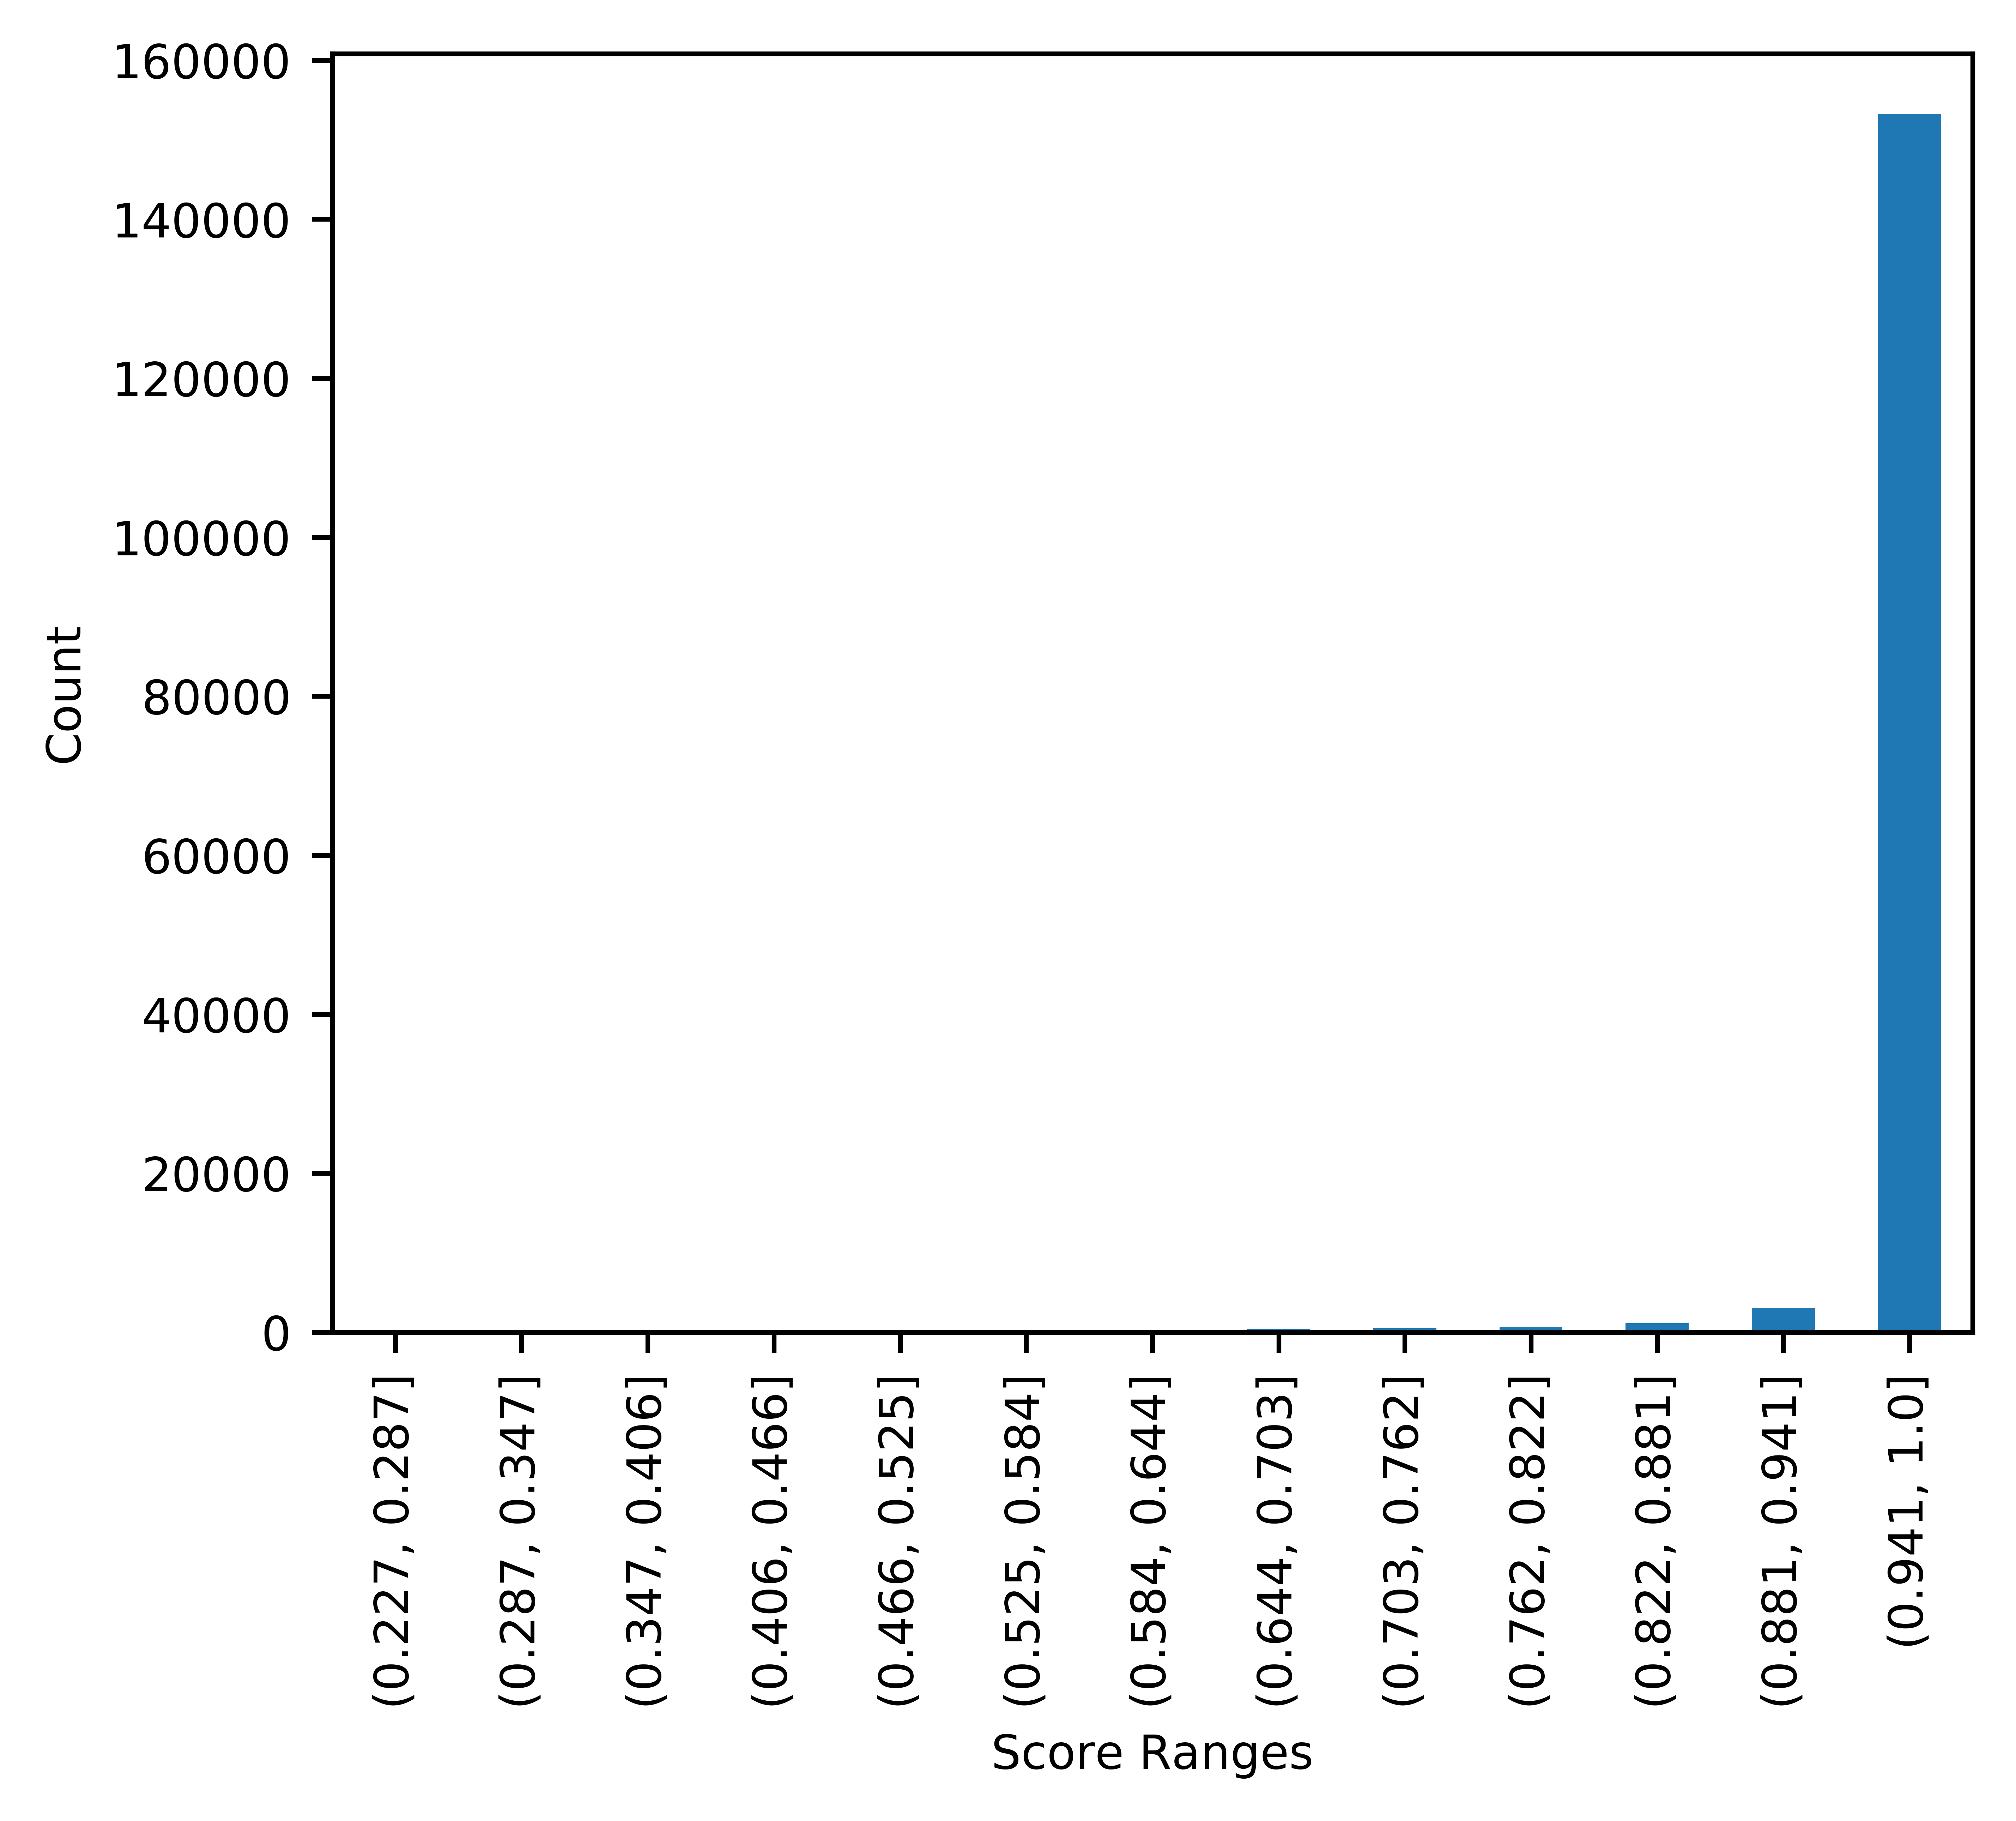
\includegraphics{./Figures/Ch_7_Results/IMG_Result_Distribution.png}
  \caption{Testing data score ranges distribution.}~\label{Fig:Results_Distribution}
\end{figure}

The second Interesting example to check how the model can understand the pattern without  \textit{Tashkeel} and the effect of adding  \textit{Tashkeel} to the text. We will take the second row from Table~\ref{Tab:Results_Article}. In the case without  \textit{Tashkeel}, the model automatically tried to find any sequences of character that follow any of the Meters patterns. The model only cared about the pattern regarding the  \textit{Tafa'il} not the mean of the text. So, we can find the model could successfully detect a sequence of characters which follow \textit{Al-Taweel} with score 0.9988. In the case with Tashkeel, the model understood the new pattern of \textit{Tafa'il} and gave the text low probability which below the threshold and classified it as non-poem (not related to the 16 classic meters) with score 0.8390. We can show how  \textit{Tashkeel} can add a feature for model understanding to the \textit{Tafa'il} pattern of the poem.


\textbf{Example:}

\begin{Arabic}
  \begin{traditionalpoem}
    يُعَدُ بُورنُموُث بَوْاْبَةُ صَلَاح للعَوْدةِ\quad & \quad للتَسْجِيلِ هَذا المُوسِمِ فيِ بريميرليجِ\\
    يعد بورنموث بوابة صلاح للعودة\quad & \quad للتسجيل هذا الموسم في بريميرليج\\

    {\color{purple} يعدبو} {\color{blue} رنموث بو} {\color{OliveGreen} ابة ص} {\color{Brown} لاح للعودة}\quad & \quad
    {\color{purple}للتسج } {\color{blue} يل هذا ال} {\color{OliveGreen} موسم في } {\color{Brown} بريميرليج}\\

    {\color{purple} \texttt{0/0//}} {\color{blue} \texttt{0/0/0//}} {\color{OliveGreen} \texttt{/0//}} {\color{Brown} \texttt{0//0//}}\quad & \quad
    {\color{purple} \texttt{0/0//}} {\color{blue} \texttt{0/0/0//}}  \texttt{{\color{OliveGreen}/0//}{\color{red}/}{\color{OliveGreen}0}} {\color{Brown} \texttt{0//0//}}\\
    {\color{purple} \texttt{0/0//}} {\color{blue} \texttt{0/0/0// }} {\color{OliveGreen} \texttt{/0//}} {\color{Brown} \texttt{0/0///}}\quad & \quad
    {\color{purple} \texttt{0/0//}} {\color{blue} \texttt{0/0/0//}} {\color{OliveGreen} \texttt{0/0//}} {\color{Brown} \texttt{0//0//}}\\
        
    {\color{purple} فَعُوْلُنْ} {\color{blue} مَفَاعِيْلُنْ} {\color{OliveGreen} فَعُولُ} {\color{Brown} مَفَاعِلُنْ}\quad & \quad
    {\color{purple} فَعُوْلُنْ} {\color{blue} مَفَاعِيْلُنْ} {\color{OliveGreen} فَعُوْلُنْ} {\color{Brown} مَفَاعِيْلُنْ}

  \end{traditionalpoem}
\end{Arabic}


\clearpage

\section{Discussion}\label{Sec:Discussion}

In this section, we need to discuss some points regarding our experiments and results approach. We will show some parts we think it needs more discussion or exploration.


\subsection{Dataset Unbalanced}

Our dataset was unbalanced which for sure affect the results we showed we have some significant drops in Per-class accuracy which most of them regarding the data size issue. We think we should have some further work regarding this point to reconstruct the experiments with balanced data, for example, 10k samples per class and check the results. Another approach could be to increase the size of the small classes to be at least 5\% of the overall classes percentage this would enhance the learning accuracy of these classes.  
\subsection{Encoding Method}

Although all the encoding methods which carry the same information should produce the same results in theory, In practice, Deep Neural Networks showed this is not the case. To explain the reason let’s first explain how Neural Network work with different encoding mechanism?

The encoding method is a transformer function $\mathcal{T}$ this function transform a discrete input values $X$. We can denote to the values as a transformed feature $\mathcal{T}(X)$ the output of this transformer method. The output $\mathcal{T}(X)$ of this transformer in the new encoding space will be input to the Neural Network model. The model should be able to ``decode''  this type of encoding. Since the lossless encoding is invertible, it is clear for any two functions and any two encodings that $\eta_1\left(\mathcal{T}_1(X)\right) = \left(\eta_1\cdot\mathcal{T}_1\cdot \mathcal{T}_2^{-1} \right)\left(\mathcal{T}_2(X)\right)$. This means that if the network $\eta_1$ is the most accurate network which can ``decode'' the encoding function (transformer) $\mathcal{T}_1$ this network $\eta_1$ is not a general network which can understand any encoding function. Also, to design this network requires a very complex architecture. So, if we have another encoding function $\mathcal{T}_2$ and we tried to use the same network for the $\mathcal{T}_2$ requires designing another network $\eta_2 = \eta_1\cdot\mathcal{T}_1\cdot \mathcal{T}_2^{-1}$. However, this network may be of complicated architecture to ``decode'' the complicated pattern of $\mathcal{T}_2(X)$.

In general, Any encoding function $\mathcal{T}$ require a special network $\eta$ to get the correct decoding (learning) for the dataset. So, our comparison between the encoding methods in the same Neural Networks architecture not accurate as each one required different network design. But all of them will reach the same results but with a different time or can be a small difference due to the not accurate network architecture. Moreover, Our work illustrated clearly the effect of the encoding methods and compared between each other, We think the \textit{Two-Hot} encoding is the more suitable method to work with character level problems. It is the middle approach between the \textit{One-Hot} which needs a huge amount of memory and the \textit{Binary} which loss some meaning in Arabic language diacritics effect.


\subsection{Weighting Loss Function}
Our weighting loss functions don’t solve the small classes issues (regardless the best model accuracy achieved with weighting loss but this is not a consistent result). The weighting loss function needs to be redesigned to solve this issue with the combination of learning rate and the batch size.

\subsection{Neural Network configurations}

During our work, we show the effect of different network configurations on the model learning and accuracy. We did a lot of experiments to find the best development architecture to make our experiments run faster and be able to do a lot of experiments. In the beginning, Out experiments took around 1.5 hours. Second, we proposed the multi-batch training to utilize parallel processing and prepare the data faster to the model as our data was huge. Then we use enhanced \textit{Cuda} LSTM cell which allows reducing our experiments time overall to be around 7-9 min per epoch based on the architecture of the network.

We also showed the effect of network layers on Learning and accuracy results. So, If we have done more experiments with more deep layers and more complex architecture it can reach more language knowledge and build a more complex model which will enhance both the Per-class accuracy and the overall accuracy.
\subsection{Model Assessment}

In our work, we proposed the overall accuracy score as the model assessment method for the results. But we need to highlight that the overall model accuracy produced from the Deep Neural Networks was very close to the overall accuracy score calculated from the confusion matrix and in some experiments it was almost the same. We also, tried different statistical ways, for example, $F_1$ score to assess our model and we find it will be the same as the model results.


%%% Local Variables:
%%% mode: latex
%%% TeX-master: "../master"
%%% TeX-engine: xetex
%%% End:
